\documentclass[11pt,reqno]{amsart}

\usepackage{amsmath,amssymb,amsthm,mathtools}
\usepackage{booktabs,array,multirow}
\usepackage{graphicx}
\usepackage[dvipsnames]{xcolor}
\usepackage{microtype}
\usepackage{enumitem}
\usepackage[margin=1.0in]{geometry}
\usepackage[colorlinks=true,linkcolor=MidnightBlue,citecolor=MidnightBlue,urlcolor=MidnightBlue]{hyperref}

\newtheorem{theorem}{Theorem}[section]
\newtheorem{proposition}[theorem]{Proposition}
\newtheorem{lemma}[theorem]{Lemma}
\newtheorem{corollary}[theorem]{Corollary}
\theoremstyle{definition}
\newtheorem{definition}[theorem]{Definition}
\theoremstyle{remark}
\newtheorem{remark}[theorem]{Remark}

\numberwithin{equation}{section}
\allowdisplaybreaks

\newcommand{\dd}{\mathrm{d}}
\newcommand{\ii}{\mathrm{i}}
\newcommand{\ee}{\mathrm{e}}
\newcommand{\RePt}{\operatorname{Re}}
\newcommand{\ImPt}{\operatorname{Im}}
\newcommand{\Li}{\mathrm{Li}}
\newcommand{\DHf}{\mathrm{DH}}
\newcommand{\defm}{\mathrm{def}}
\newcommand{\tri}{\mathrm{tri}}
\newcommand{\sq}{\mathrm{sq}}
\newcommand{\corn}{\mathrm{corn}}
\newcommand{\dual}{\mathrm{dual}}

\begin{document}
\sloppy

\title[The Chladni Portal-Frame Synthesis for Riemann's $\Xi$-Function]{The Chladni Portal-Frame Synthesis: Codimension-Three Saddle Overdetermination, Green--Dirichlet--Neumann Chamber Equipartition, and Euler Dilogarithm $\mathrm{Li}_2(2\theta)$ Horizon Damping for Riemann's $\Xi$-Function}

\author{Thijs Missiaen}
\address{Independent Researcher, Belgium}
\email{thijs.missiaen@gmail.com}
\thanks{2020 \emph{Mathematics Subject Classification.} Primary 11M06, 11M26; Secondary 30D15, 31A05, 33B30.\\
\emph{Key words and phrases.} Riemann Xi-function, Chladni nodal chambers, portal-frame dichotomy, codimension-three saddle overdetermination, Green--Dirichlet--Neumann equipartition, Wronskian--slope reciprocity, Euler dilogarithm, Dirichlet hyperbola method.\\
ORCID: \href{https://orcid.org/0009-0007-3678-0810}{0009-0007-3678-0810}. Competing interests: The author declares no competing financial or non-financial interests.}

\dedicatory{\upshape October 25, 2026}
\date{October 25, 2026}

\begin{abstract}
We unify the macro-, meso-, and micro-scale Cauchy--Riemann geometry of Riemann's completed zeta function $\Xi(t-\ii d)=R(d,t)+\ii I(d,t)$ ($d\ge 0$) around a harmonic Chladni nodal chamber $\Omega_k(d_0)$. At the macro-scale, we prove that any off-critical zero on a transverse Chladni wall $I(d,t)=0$ is governed by an exact dichotomy between a critical-line Laguerre defect $c_1(\tau_*)=-\Xi(\tau_*)\Xi''(\tau_*)\le 0$ and a codimension-three interior saddle overdetermination $\{I=\partial_d I=\partial_t I=0\}$ ($3$ real equations in $2$ unknowns), with $100\%$ of the first five off-critical zeros of the Davenport--Heilbronn counterexample $\Xi_{\DHf}(z)$ forced into the critical-line defect case. At the meso-scale, Green's first identity enforces an exact $50\%$--$50\%$ Dirichlet--Neumann boundary-flux equipartition $\int R\,\partial_d R\,\dd t \equiv \int I\,\partial_d I\,\dd t \equiv \iint_{\Omega_k}|\Xi'|^2\,\dd d\,\dd t = \frac{1}{2}\mathcal{W}_{\Omega_k}(d_0)>0$ coupled with the Wronskian--slope reciprocity $\tau_k'(d)\equiv R\,\partial_t R/(d\,\widetilde{W})$. At the micro-scale, Euler dilogarithm $\Li_2(2\theta)$ horizon damping raises the quadratic Wronskian forward-triangle capture fraction at $\theta=1/6$ from $\eta^{(0)}(1/6)=0.243955$ to $\eta^{(2)}(1/6)=0.676891>2/3>1/2$ ($\Delta(\eta^{(2)}(1/6))=-0.353781<0$) with fourth-order Dirichlet hyperbola apex pinching $(\omega_p\omega_q)^2\le \frac{1}{16}(\ln m_{\dual})^4$.
\end{abstract}

\maketitle

\section{Introduction, Resolved Bottlenecks, and the Three-Scale Portal-Frame Architecture}\label{sec:intro}

Let $\xi(s) = \frac{1}{2}s(s-1)\pi^{-s/2}\Gamma(s/2)\zeta(s)$ denote Riemann's completed zeta function, and define the real-on-real entire function of order one
\begin{equation}\label{eq:Xi-def}
\Xi(z) := \xi\Bigl(\frac{1}{2} + \ii z\Bigr) = \int_0^\infty \Phi(u)\cos(zu)\,\dd u, \qquad z = t - \ii d, \quad d = \sigma - \frac{1}{2} \ge 0,
\end{equation}
where $\Phi(u) = \sum_{n=1}^\infty (2\pi^2 n^4 \ee^{9u/2} - 3\pi n^2 \ee^{5u/2})\exp(-\pi n^2 \ee^{2u}) > 0$ is Riemann's super-exponentially decaying kernel \cite{Riemann1859,Titchmarsh1986}. Decomposing $\Xi(t-\ii d)$ into its real and imaginary parts on the closed right half-strip $d \ge 0$,
\begin{equation}\label{eq:R-I-def}
\Xi(t - \ii d) = R(d,t) + \ii I(d,t), \qquad R(0,t) = \Xi(t), \quad I(0,t) \equiv 0,
\end{equation}
transforms the location of complex zeros of $\zeta(s)$ into a boundary-value problem for two conjugate harmonic fields $(R,I)$ satisfying the Cauchy--Riemann system $\partial_d R = \partial_t I$ and $\partial_t R = -\partial_d I$ \cite{Jensen1913,Polya1926,Speiser1934}. Because $I(0,t) \equiv 0$ identically along the critical line $d=0$, the zero locus $\{I(d,t)=0\}$ forms a rigid architectural skeleton consisting of the vertical spine $d=0$ and transverse \emph{Chladni nodal walls} $\Gamma_k = \{(d,\tau_k(d)) : d \ge 0\}$ branching orthogonally off the critical line at the real extrema $\tau_k(0)$ where $\Xi'(\tau_k(0))=0$ \cite{Missiaen2026P2,Missiaen2026P8,Missiaen2026P13}. Two consecutive walls $\Gamma_k$ and $\Gamma_{k+1}$, together with the critical-line floor $\{0\} \times [\tau_k(0),\tau_{k+1}(0)]$ and a vertical right-hand cutoff $\{d_0\} \times [\tau_k(d_0),\tau_{k+1}(d_0)]$, enclose a harmonic \emph{Chladni nodal chamber} (or \emph{portal frame}) $\Omega_k(d_0)$.

In the preceding thirteen papers of this series \cite{Missiaen2026P1,Missiaen2026P2,Missiaen2026P3,Missiaen2026P4,Missiaen2026P5,Missiaen2026P6,Missiaen2026P7,Missiaen2026P8,Missiaen2026P9,Missiaen2026P10,Missiaen2026P11,Missiaen2026P12,Missiaen2026P13}, we developed the transverse Wronskian calculus, the exact parity-reduced energy identity $W(d,t) \equiv 2d\,\widetilde{W}(d,t)$, the finite Euler-product prime gauge $\mathcal{P}_{\le X}(s)$, and the second-order de Branges phase-velocity lifting theorem. Despite these advances, three foundational structural questions remained open across the macro-, meso-, and micro-scales of a Chladni portal frame $\Omega_k(d_0)$:
\begin{enumerate}[label=(\roman*),leftmargin=2.2em]
\item \textbf{Macro-Scale Wall-Zero and Saddle Bottleneck:} Since every point on a Chladni wall $\Gamma_k$ already satisfies $I(d,t)=0$, an off-critical zero $z_* = \gamma_* - \ii d_*$ ($d_* > 0$) occurs precisely where $R(d,t)$ changes sign along a wall. What prevents a wall $\Gamma_k$ from losing its critical-line real amplitude $|R(0,\tau_k(0))| > 0$ and crossing $R=0$ in the interior $d>0$, either directly from $d=0$ or via a hyperbolic saddle bifurcation $\Xi'(z_c)=0$ in $d>0$?
\item \textbf{Meso-Scale Chamber Flux and Wronskian--Slope Bottleneck:} Inside a chamber $\Omega_k(d_0)$ bounded by curved walls $\tau_k(d)$ and $\tau_{k+1}(d)$, how is the vertical boundary flux $\int [R\,\partial_d R + I\,\partial_d I]\,\dd t$ partitioned between the real field $R$ and the imaginary field $I$, and how does the geometric bending slope $\tau_k'(d)$ of a Chladni wall interact with the reduced transverse Wronskian $\widetilde{W}(d,t)$ when comparing genuine Euler-product $L$-functions against counterexamples such as the Davenport--Heilbronn function $\Xi_{\DHf}(z)$ \cite{DavenportHeilbronn1936}?
\item \textbf{Micro-Scale Quadratic Semiprime Anti-Phase and Reflection Bottleneck:} At high spectral height $t \gg 1$, when the prime gauge $\mathcal{P}_{\le X}(s)$ is truncated at the cubic-window threshold $X = N_\star(t)^{2\theta}$ with $\theta = 1/6$ ($N_\star(t) = \sqrt{t/(2\pi)}$), the unattenuated quadratic expansion $|1 + U + U^2/2|^2$ along the anti-phase axis $V = \ImPt\,\mathcal{P}_{>X}(s)=0$ drops from $1$ to $1/2$ at $U=-1$, while the unweighted forward-triangle capture fraction of the semiprime square $(X,N_\star]^2$ is only $\eta^{(0)}(1/6) = 0.243955 < 1/2$. How does the Riemann--Siegel horizon $pq \le N_\star(t)$, combined with the second-order Wronskian weight $\omega_n(t)^2 = \ln^2(N_\star^2/n^2)$, restore a strictly positive quadratic discriminant floor and suppress the reflected corner $pq > N_\star(t)$?
\end{enumerate}

The purpose of this flagship fourteenth paper is to resolve all three questions within a single, organically interlocked mathematical synthesis across the macro-, meso-, and micro-scales of the Chladni portal frame $\Omega_k(d_0)$. Our central synthesis result is stated as follows.

\begin{theorem}[The Three-Scale Chladni Portal-Frame and Dilogarithm Horizon Synthesis]\label{thm:main-synthesis}
Let $F(z)$ be any real-entire function in the Riemann--Hecke class satisfying $F(\bar{z})=\overline{F(z)}$, and write $F(t-\ii d) = R(d,t) + \ii I(d,t)$ for $d \ge 0$, $t \in \mathbb{R}$, with critical-line Laguerre curvature functional $c_1(t) := (F'(t))^2 - F(t)F''(t)$ and reduced transverse Wronskian
\begin{equation}\label{eq:W-tilde-intro}
\widetilde{W}(d,t) := \frac{R(d,t)\,\partial_t I(d,t) - I(d,t)\,\partial_t R(d,t)}{d}, \qquad \lim_{d \to 0^+} \widetilde{W}(d,t) = c_1(t).
\end{equation}
Then the following three interlocked structural laws hold across the macro-, meso-, and micro-scales:
\begin{enumerate}[label=\upshape(\Roman*),leftmargin=2.4em]
\item \textbf{Macro-Scale Portal-Frame Dichotomy and Codimension-Three Saddle Overdetermination (Section~\ref{sec:macro}):} Along any smooth segment of the Chladni nodal locus $\{I(d,t)=0\}$, the tangential Cauchy--Riemann derivative of $R$ equals $\dd R/\dd s = \pm |\nabla I| = \pm |F'(t-\ii d)|$, and no connected component of $\{I=0\} \cap \{d>0\}$ can form a closed loop or a two-footed arch returning to $d=0$. At any simple critical-line extremum $\tau_*$ ($F'(\tau_*)=0$, $F(\tau_*)\ne 0$), the transverse wall curvature and critical-line curvature obey the exact harmonic conservation law
\begin{equation}\label{eq:harmonic-conservation-intro}
\frac{1}{2}\frac{\dd^2}{\dd d^2}\Bigl[\bigl|R(d,\tau_*(d))\bigr|^2\Bigr]_{d=0} = -\frac{1}{2}\frac{\dd^2}{\dd t^2}\Bigl[F(t)^2\Bigr]_{t=\tau_*} = -F(\tau_*)F''(\tau_*) = c_1(\tau_*).
\end{equation}
Consequently, an off-critical zero $z_* = \gamma_* - \ii d_*$ ($d_* > 0$) on a Chladni wall $\Gamma_*$ can arise if and only if either \emph{(Case~I)} the critical-line anchor violates Laguerre--P\'{o}lya convexity via $c_1(\tau_*) \le 0$, or \emph{(Case~II)} $\Gamma_*$ undergoes an interior saddle bifurcation in $d>0$ satisfying the codimension-three overdetermined system $I(d_c,t_c) = \partial_d I(d_c,t_c) = \partial_t I(d_c,t_c) = 0$ ($3$ real equations in $2$ real unknowns, versus $1$ equation in $1$ unknown on $d=0$).
\item \textbf{Meso-Scale $50\%$--$50\%$ Chamber Equipartition and Wronskian--Slope Reciprocity (Section~\ref{sec:meso}):} On every regular Chladni chamber $\Omega_k(d_0)$ bounded by $0 < d < d_0$ and $\tau_k(d) < t < \tau_{k+1}(d)$, the curved Dirichlet side walls $I=0$ and Neumann critical-line floor $I=0$, $\partial_d R=0$ enforce an exact $50\%$--$50\%$ Green--Dirichlet--Neumann boundary-flux equipartition:
\begin{equation}\label{eq:equipartition-intro}
\int_{\tau_k(d_0)}^{\tau_{k+1}(d_0)} R(d_0,t)\,\partial_d R(d_0,t)\,\dd t \equiv \int_{\tau_k(d_0)}^{\tau_{k+1}(d_0)} I(d_0,t)\,\partial_d I(d_0,t)\,\dd t \equiv \iint_{\Omega_k(d_0)} \bigl|F'(t-\ii d)\bigr|^2\,\dd d\,\dd t > 0,
\end{equation}
while along each bounding Chladni wall $\Gamma_k = \{(d,\tau_k(d))\}$, the geometric wall slope $\tau_k'(d)$, the reduced Wronskian $\widetilde{W}$, and the wall amplitude $R(d,\tau_k(d))$ satisfy the exact reciprocity identities
\begin{equation}\label{eq:reciprocity-intro}
\tau_k'(d) \equiv \frac{R\,\partial_t R}{d\,\widetilde{W}}\Big|_{\Gamma_k}, \qquad 1 + \tau_k'(d)^2 \equiv \frac{R^2\,\bigl|F'\bigr|^2}{d^2\,\widetilde{W}^2}\Big|_{\Gamma_k}, \qquad \frac{\dd}{\dd d}\Bigl[\frac{1}{2}R\bigl(d,\tau_k(d)\bigr)^2\Bigr] \equiv d\,\widetilde{W}\,\bigl(1 + \tau_k'(d)^2\bigr).
\end{equation}
\item \textbf{Micro-Scale Euler Dilogarithm $\Li_2(2\theta)$ Horizon Damping and Dirichlet Hyperbola Reflection Duality (Section~\ref{sec:micro}):} For $F=\Xi$ at spectral height $t \gg 1$ with saddle horizon $N_\star(t)=\sqrt{t/(2\pi)}$ and sieve cutoff $X = N_\star^{2\theta}$ ($\theta \in (0,1/4)$), splitting the quadratic semiprime tail $\frac{1}{2}\mathcal{P}_{>X}(s)^2 = \mathcal{T}_{\le N_\star}(s) + \mathcal{C}_{>N_\star}(s)$ across the Dirichlet hyperbola $pq = N_\star(t)$ yields an attenuated quadratic spring $|1 + U + \frac{\eta}{2}U^2|^2 \ge (1 - \frac{1}{2\eta})^2 > 0$ with negative discriminant $\Delta(\eta) = 1 - 2\eta < 0$ whenever the forward-triangle capture fraction $\eta = \eta^{(p)}(\theta)$ exceeds $1/2$. Under $p$-th order logarithmic horizon weighting $\omega_n(t)^p = \ln^p(N_\star^2/n^2)$, $\eta^{(p)}(\theta)$ is given in exact closed form by Euler's dilogarithm $\Li_2(2\theta)$ (Theorem~\ref{thm:dilogarithm-laws}), raising the capture fraction at the cubic-window threshold $\theta=1/6$ from $\eta^{(0)}(1/6)=0.243955 < 1/2$ to $\eta^{(2)}(1/6) = 0.676891 > 2/3 > 1/2$ and $\eta^{(3)}(1/6) = 0.798091$, while the reflected corner $pq > N_\star(t)$ satisfies the exact reflection law $\omega_p(t)+\omega_q(t) \equiv \ln m_{\dual}(pq)$ and fourth-order apex pinching $(\omega_p\omega_q)^2 \le \frac{1}{16}(\ln m_{\dual})^4 \to 0$ as $pq \to N_\star(t)^2$.
\end{enumerate}
\end{theorem}

The fundamental constants governing this three-scale synthesis are certified to $65$ decimal places in our verification suite and take the following canonical values at the cubic-window threshold $\theta = 1/6$ ($\tau = 2\theta = 1/3$) and the first Davenport--Heilbronn counterexample chamber $t \in [83.89, 86.63]$:
\begin{equation}\label{eq:canonical-constants}
\begin{aligned}
\eta^{(0)}(1/6) &= 0.2439550996 < 1/2, &\quad \eta^{(2)}(1/6) &= 0.6768906167 > 2/3 > 1/2, \\
\eta^{(3)}(1/6) &= 0.7980906218 > 3/4, &\quad \Delta\bigl(\eta^{(2)}(1/6)\bigr) &= 1 - 2\eta^{(2)}(1/6) = -0.3537812333 < 0, \\
\theta_{*,50\%}^{(2)} &= 0.1905498467 > \theta_{\mathrm{W\text{-}pure}}^\infty, &\quad (d_{\mathrm{tip}}, t_{\mathrm{tip}})_{\DHf} &= (0.2980980120,\, 85.6254944428).
\end{aligned}
\end{equation}

\subsection{Proof overview}\label{subsec:proof-overview}

The architecture of this paper is designed so that Sections~\ref{sec:macro}, \ref{sec:meso}, and \ref{sec:micro} form one continuous, deductive chain from the global topology of $\Omega_k(d_0)$ down to individual prime-pair interactions across the Riemann--Siegel saddle horizon:
\begin{enumerate}[label=\textbf{Step \arabic*.},leftmargin=4.2em]
\item \textbf{From Global Chladni Topology to Boundary-to-Interior Curvature Conservation (Section~\ref{sec:macro}):} We begin on the macro-scale by applying the Cauchy--Riemann equations along arc length $s$ of any zero contour $I(d,t)=0$, obtaining $\dd R/\dd s = \pm|\nabla I| = \pm|\Xi'|$. Because $I(d,t)$ is harmonic on $\mathbb{R}^2$ and vanishes identically on $d=0$, the Harmonic Maximum Principle prohibits any closed loop or two-footed arch of $\{I=0\}$ in $d>0$. Differentiating $R(d,\tau_*(d))^2$ twice with respect to $d$ at a critical-line anchor $\tau_*$ where $\Xi'(\tau_*)=0$ reveals the conservation law \eqref{eq:harmonic-conservation-intro}: the transverse wall acceleration at $d=0$ is equal and opposite to the critical-line longitudinal curvature $\frac{1}{2}\partial_t^2[\Xi(t)^2]_{t=\tau_*}$, and both equal $c_1(\tau_*)$. Thus, if $c_1(\tau_*)>0$, $|R|$ initially grows quadratically away from $d=0$. For $|R|$ to reverse course and vanish in $d>0$, the wall must encounter a complex zero of $\Xi'(z)$, which requires solving the codimension-three system $\{I=\partial_d I=\partial_t I=0\}$ ($3$ equations in $2$ unknowns). In Theorem~\ref{thm:dh-case1-equivalence}, we prove that when the Euler product is broken (as in $\Xi_{\DHf}$), off-critical zeros are forced into \emph{Case~I} ($c_1^{\DHf}(\tau_{\mathrm{false},m}) < 0$ on $d=0$), and that under the P\'{o}lya--Jensen--Speiser derivative condition, zero-freeness in $d>0$ is strictly equivalent to $1$D critical-line positivity $c_1(t)>0$.
\item \textbf{From Macro-Scale Walls to Meso-Scale Chamber Equipartition and Slope Reciprocity (Section~\ref{sec:meso}):} Having established that the walls $\Gamma_k$ and $\Gamma_{k+1}$ bound a well-defined portal frame $\Omega_k(d_0)$, Section~\ref{sec:meso} zooms into the meso-scale interior of $\Omega_k(d_0)$. Applying Green's first identity separately to $(R,\Delta R=0)$ and $(I,\Delta I=0)$ on $\Omega_k(d_0)$ shows that the curved side walls $\Gamma_k,\Gamma_{k+1}$ act as homogeneous Dirichlet boundaries ($I=0$) for the $I$-integral and, simultaneously, via the tangential Cauchy--Riemann law $\partial_n R = \pm \partial_s I = 0$, as homogeneous Neumann boundaries ($\partial_n R = 0$) for the $R$-integral. This dual Dirichlet--Neumann cancellation annihilates all side-wall and floor boundary contributions for both fields, proving that $R$ and $I$ each carry \emph{exactly $50\%$} of the total $2$D Wronskian flux $\mathcal{W}_{\Omega_k}(d_0)$ across the vertical cutoff $d=d_0$ (Theorem~\ref{thm:green-equipartition}). Differentiating $I(d,\tau_k(d))\equiv 0$ along the wall then links the wall slope $\tau_k'(d)$ and wall amplitude growth $\frac{\dd}{\dd d}(\frac{1}{2}R^2)$ directly to the meso-scale reduced Wronskian $\widetilde{W}(d,t)$ via \eqref{eq:reciprocity-intro} (Theorem~\ref{thm:wronskian-slope-reciprocity}), explaining why the detached real nodal parabola $R_{\DHf}=0$ of Davenport--Heilbronn suffers a vertical fold singularity $|t_R'(d_{\mathrm{tip}})|=\infty$ precisely where $\widetilde{W}_{\DHf}(d_{\mathrm{tip}},t_{\mathrm{tip}})=0$.
\item \textbf{From Meso-Scale Wronskian Weighting to Micro-Scale $\Li_2(2\theta)$ Horizon Damping (Section~\ref{sec:micro}):} Finally, Section~\ref{sec:micro} asks: \emph{why} does the meso-scale Wronskian $\widetilde{W}$ remain positive for Euler-product $L$-functions across the quadratic semiprime anti-phase regime where $U = \RePt\,\mathcal{P}_{>X}(s) < 0$? At the micro-scale, the Riemann--Siegel stationary-phase saddle $N_\star(t)=\sqrt{t/(2\pi)}$ splits the quadratic prime-pair sum $\frac{1}{2}\mathcal{P}_{>X}(s)^2$ into a forward triangle $\mathcal{T}_{\le N_\star}(s)$ ($pq \le N_\star$) and a reflected corner $\mathcal{C}_{>N_\star}(s)$ ($pq > N_\star$). Because the meso-scale Wronskian acts as a second-order differential operator on $\Xi$, each prime $n$ carries the intrinsic logarithmic horizon weight $\omega_n(t) = \ln(N_\star^2/n^2) = L(1-2\alpha)$ under the quadratic Wronskian ($p=2$). Integrating $(1-2\alpha_1)^p(1-2\alpha_2)^p$ over the simplex $\alpha_1+\alpha_2 \le 1/2$ inside $[\theta,1/2]^2$ yields the exact Euler dilogarithm laws $\eta^{(p)}(\theta)$ in Theorem~\ref{thm:dilogarithm-laws}, proving that Wronskian weighting flips the quadratic semiprime polynomial from an under-damped real-root regime ($\eta^{(0)}(1/6)=0.2440 < 1/2$) into an over-damped complex-conjugate root regime ($\eta^{(2)}(1/6)=0.6769 > 2/3 > 1/2$), while Theorem~\ref{thm:hyperbola-duality} proves fourth-order pinching of the reflected corner at the horizon apex $pq=N_\star^2$.
\end{enumerate}

\subsection{Notation and conventions}\label{subsec:notation}

Throughout this paper, $s = \sigma + \ii t = \frac{1}{2} + d + \ii t$ denotes the complex spectral variable, and $z = -\ii(s - \frac{1}{2}) = t - \ii d$ denotes the rotated variable in which the critical line $\sigma=1/2$ coincides with the real axis $d=0$. For any real-entire function $F(z)$ satisfying $F(\bar{z})=\overline{F(z)}$, we write $F(t-\ii d) = R(d,t) + \ii I(d,t)$, where $R(d,t)=\RePt\,F(t-\ii d)$ is even in $d$ and $I(d,t)=\ImPt\,F(t-\ii d)$ is odd in $d$. The $1$D critical-line Laguerre functional is $c_1(t) := (F'(t))^2 - F(t)F''(t)$, and its $2$D continuation is the transverse Wronskian $W(d,t) := 2(R\,\partial_t I - I\,\partial_t R) = 2(R\,\partial_d R + I\,\partial_d I) \equiv 2d\,\widetilde{W}(d,t)$, where $\widetilde{W}(d,t) = (R\,\partial_t I - I\,\partial_t R)/d$ satisfies $\lim_{d\to 0^+}\widetilde{W}(d,t) = c_1(t)$ (see Remark~\ref{rem:normalization}). For polylogarithms, $\Li_2(x) := \sum_{k=1}^\infty x^k/k^2 = -\int_0^x \ln(1-u)\,u^{-1}\,\dd u$ denotes Euler's dilogarithm for $x < 1$ \cite{Lewin1981}. At spectral height $t > 2\pi$, $N_\star(t) := \sqrt{t/(2\pi)}$ denotes the continuous Riemann--Siegel horizon, $L := \ln N_\star(t) = \frac{1}{2}\ln(t/(2\pi))$, and $\omega_n(t) := 2\ln(N_\star(t)/n) = L(1 - 2\alpha_n)$ denotes the logarithmic saddle distance of an integer $n$ with logarithmic scale $\alpha_n := (\ln n)/L$.

\section{Portal-Frame Topological Dichotomy, Harmonic Curvature Conservation, and Codimension-Three Saddle Overdetermination}\label{sec:macro}

We begin at the macro-scale by analyzing the global nodal geometry of the harmonic fields $R(d,t)$ and $I(d,t)$ in the closed right half-plane $d \ge 0$. Because $I(0,t) \equiv 0$, every simple real extremum $\tau_k(0)$ of $\Xi(t)$ on the critical line ($\Xi'(\tau_k(0))=0$, $\Xi''(\tau_k(0))\ne 0$) is a saddle point of $I(d,t)$ from which a unique transverse Chladni nodal wall $\Gamma_k$ bifurcates orthogonally into $d > 0$ \cite{Missiaen2026P2,Missiaen2026P8}. Our first theorem establishes the exact differential-geometric laws along $\Gamma_k$, rules out closed loops and returning arches in $d \ge 0$, proves the boundary-to-interior harmonic curvature conservation law, and classifies the exact dichotomy for any hypothetical off-critical zero.

\begin{theorem}[Portal-Frame Topological Dichotomy and Codimension-Three Saddle Overdetermination]\label{thm:portal-dichotomy}
Let $F(z)$ be a non-constant real-entire function of finite order with $F(t-\ii d)=R(d,t)+\ii I(d,t)$. Then:
\begin{enumerate}[label=\upshape(\alph*),leftmargin=2.2em]
\item \textbf{Tangential Cauchy--Riemann Monotonicity Law:} Let $\Gamma \subset \{I(d,t)=0\}$ be any regular arc of the imaginary nodal locus parameterized by Euclidean arc length $s$ with unit tangent vector $\mathbf{T} = (d'(s),t'(s))$ and unit normal $\mathbf{N} = (-t'(s),d'(s))$. Along $\Gamma$, the tangential derivative of $R$ and the normal derivative of $R$ satisfy
\begin{equation}\label{eq:tangential-CR}
\frac{\dd}{\dd s}R\bigl(d(s),t(s)\bigr) = \pm \bigl|\nabla I\bigl(d(s),t(s)\bigr)\bigr| = \pm \bigl|F'\bigl(t(s)-\ii d(s)\bigr)\bigr|, \qquad \frac{\partial R}{\partial n}\Big|_\Gamma = 0.
\end{equation}
In particular, $R(d(s),t(s))$ is strictly monotonic along any arc of $\{I=0\}$ free of complex derivative zeros $F'(z)=0$.
\item \textbf{Topological Exclusion of Loops and Returning Arches:} No connected bounded component of $\{d>0\} \setminus \{I(d,t)=0\}$ can have boundary contained entirely within $\{I(d,t)=0\} \cup \{d=0\}$. Consequently, the Chladni locus $\{I(d,t)=0\}$ cannot form any closed loop in $d>0$, nor can any Chladni wall $\Gamma_k$ emanating from $(0,\tau_k(0))$ bend back to terminate at another critical-line anchor $(0,\tau_j(0))$ to form a bounded two-footed arch over $d=0$.
\item \textbf{Harmonic Curvature Conservation Law:} Let $\tau_* \in \mathbb{R}$ be a critical-line anchor where $F'(\tau_*)=0$ and $F(\tau_*)\ne 0$, and let $\Gamma_* = \{(d,\tau_*(d))\}$ be the transverse Chladni wall emanating from $(0,\tau_*)$. Then at $(d,t)=(0,\tau_*)$,
\begin{equation}\label{eq:harmonic-curvature-conservation}
\frac{1}{2}\frac{\dd^2}{\dd d^2}\Bigl[\bigl|R\bigl(d,\tau_*(d)\bigr)\bigr|^2\Bigr]_{d=0} = -\frac{1}{2}\frac{\dd^2}{\dd t^2}\Bigl[F(t)^2\Bigr]_{t=\tau_*} = -F(\tau_*)F''(\tau_*) = c_1(\tau_*),
\end{equation}
with the local Taylor expansion along $\Gamma_*$ given by
\begin{equation}\label{eq:wall-taylor}
\bigl|R\bigl(d,\tau_*(d)\bigr)\bigr|^2 = F(\tau_*)^2 + c_1(\tau_*)\,d^2 + O(d^4) \qquad (d \to 0^+).
\end{equation}
\item \textbf{Exact Wall-Zero Dichotomy and Codimension-Three Overdetermination:} Suppose $F(z_*)=0$ at an off-critical point $z_* = \gamma_* - \ii d_*$ with $d_* > 0$, lying on a connected component $\Gamma_*$ of $\{I(d,t)=0\} \cap \{d>0\}$ that meets the critical line at $(0,\tau_*)$ with $F(\tau_*)\ne 0$. Then at least one of the following two mutually supplementary mechanisms must occur:
\begin{itemize}[leftmargin=1.8em]
\item \textbf{Case~I (Critical-Line Laguerre Convexity Breakdown):} The critical-line anchor violates Laguerre--P\'{o}lya convexity,
\begin{equation}\label{eq:case-I}
c_1(\tau_*) = -F(\tau_*)F''(\tau_*) \le 0 \quad \Longleftrightarrow \quad F(\tau_*)F''(\tau_*) \ge 0,
\end{equation}
so that $|R(d,\tau_*(d))|$ decreases from $d=0$ directly toward $R(d_*,\gamma_*)=0$ without requiring any interior critical point of $F$ in $d>0$.
\item \textbf{Case~II (Interior Codimension-Three Saddle Bifurcation):} The critical-line anchor satisfies $c_1(\tau_*)>0$, so $|R(d,\tau_*(d))|$ initially increases with $d$, and $\Gamma_*$ must pass through or bifurcate at an interior complex critical point $z_c = t_c - \ii d_c$ ($d_c > 0$) satisfying the simultaneous real system
\begin{equation}\label{eq:codim-3-system}
\left\{\begin{aligned}
I(d_c,t_c) &= 0, \\
\partial_d I(d_c,t_c) &= 0, \\
\partial_t I(d_c,t_c) &= 0,
\end{aligned}\right.
\end{equation}
which constitutes $3$ real equations in $2$ real unknowns $(d_c,t_c) \in (0,\infty)\times\mathbb{R}$ (codimension $3$ in the $2$D half-plane, hence structurally unstable under generic $1$-parameter deformations), whereas on the critical line $d=0$ the reflection symmetry $I(0,t)\equiv \partial_t I(0,t)\equiv 0$ reduces \eqref{eq:codim-3-system} to the single determined equation $\partial_d I(0,\tau_*)=F'(\tau_*)=0$ ($1$ equation in $1$ unknown).
\end{itemize}
\end{enumerate}
\end{theorem}

\begin{proof}
(a) Along any smooth curve $\Gamma \subset \{I(d,t)=0\}$ parameterized by arc length $s$, differentiating $I(d(s),t(s)) \equiv 0$ gives $\nabla I \cdot \mathbf{T} = \partial_d I\,d'(s) + \partial_t I\,t'(s) = 0$. Since $|\mathbf{T}|^2 = d'(s)^2 + t'(s)^2 = 1$, the gradient $\nabla I = (\partial_d I, \partial_t I)$ is collinear with the unit normal $\mathbf{N} = (-t'(s),d'(s))$, so $(\partial_d I, \partial_t I) = \pm |\nabla I|\,(-t'(s),d'(s))$. Applying the Cauchy--Riemann equations $\partial_d R = \partial_t I$ and $\partial_t R = -\partial_d I$, the tangential derivative of $R$ along $\Gamma$ is
\[
\frac{\dd}{\dd s}R\bigl(d(s),t(s)\bigr) = \partial_d R\,d'(s) + \partial_t R\,t'(s) = \partial_t I\,d'(s) - \partial_d I\,t'(s) = \nabla I \cdot \mathbf{N} = \pm \bigl|\nabla I\bigl(d(s),t(s)\bigr)\bigr|.
\]
Since $|F'(t-\ii d)|^2 = (\partial_t R)^2 + (\partial_t I)^2 = (-\partial_d I)^2 + (\partial_t I)^2 = |\nabla I|^2$, the first identity in \eqref{eq:tangential-CR} follows. Similarly, the normal derivative of $R$ along $\Gamma$ is $\partial_n R = \nabla R \cdot \mathbf{N} = -\partial_d R\,t'(s) + \partial_t R\,d'(s) = -(\partial_t I\,t'(s) + \partial_d I\,d'(s)) = -\dd I/\dd s = 0$, proving the second identity in \eqref{eq:tangential-CR}.

(b) Suppose toward a contradiction that $D \subset \{d > 0\}$ is a non-empty bounded open domain whose boundary $\partial D$ is contained in $\{I(d,t)=0\} \cup \{d=0\}$. Because $I(0,t) \equiv 0$ on the critical line, $I(d,t)$ vanishes identically on the entire boundary $\partial D$. Since $I(d,t) = \ImPt\,F(t-\ii d)$ is harmonic on $\mathbb{R}^2$, the Harmonic Maximum and Minimum Principles imply $I(d,t) \equiv 0$ throughout $D$, and by real-analyticity $I \equiv 0$ on $\mathbb{R}^2$, contradicting that $F$ is non-constant. This rules out both closed loops of $\{I=0\}$ in $d>0$ and bounded two-footed arches returning to $d=0$.

(c) Near a simple critical-line extremum $\tau_*$ ($F'(\tau_*)=0$, $F''(\tau_*)\ne 0$), expand $F(t-\ii d)$ in powers of $(t-\tau_*) - \ii d$:
\[
R(d,t) = F(\tau_*) + \frac{1}{2}F''(\tau_*)\bigl((t-\tau_*)^2 - d^2\bigr) + O\bigl((t-\tau_*)^3 + d^3\bigr),
\]
\[
I(d,t) = -d\Bigl[F''(\tau_*)(t-\tau_*) + \frac{1}{6}F^{(3)}(\tau_*)\bigl(3(t-\tau_*)^2 - d^2\bigr) + O\bigl((t-\tau_*)^3 + d^3\bigr)\Bigr].
\]
Dividing $I(d,t)=0$ by $d>0$ and applying the Implicit Function Theorem gives the unique transverse branch $\tau_*(d) = \tau_* + \frac{F^{(3)}(\tau_*)}{6F''(\tau_*)}d^2 + O(d^4)$, so $\tau_*'(0)=0$. Substituting $t = \tau_*(d)$ into $R(d,t)$ yields $R(d,\tau_*(d)) = F(\tau_*) - \frac{1}{2}F''(\tau_*)d^2 + O(d^4)$. Squaring both sides and using $F'(\tau_*)=0$ gives
\[
\bigl|R\bigl(d,\tau_*(d)\bigr)\bigr|^2 = F(\tau_*)^2 - F(\tau_*)F''(\tau_*)\,d^2 + O(d^4) = F(\tau_*)^2 + c_1(\tau_*)\,d^2 + O(d^4).
\]
On the other hand, along the critical line $d=0$, $\frac{1}{2}\partial_t^2[F(t)^2]_{t=\tau_*} = [(F'(t))^2 + F(t)F''(t)]_{t=\tau_*} = F(\tau_*)F''(\tau_*) = -c_1(\tau_*)$, which establishes \eqref{eq:harmonic-curvature-conservation} and \eqref{eq:wall-taylor}. Note that at a simple zero of $F'$ along $\Gamma_*$, $\partial_d R = \partial_t I = 0$ and $\partial_d^2 R = -\partial_t^2 R$ by Laplace's equation $\Delta R = 0$, which is the underlying harmonic source of the sign reversal between $\partial_d^2(R^2)$ and $\partial_t^2(F^2)$.

(d) Suppose $z_* = \gamma_* - \ii d_*$ ($d_* > 0$) is an off-critical zero of $F$ lying on the wall component $\Gamma_*$ anchored at $(0,\tau_*)$ with $F(\tau_*)\ne 0$. At $d=0$, $|R(0,\tau_*)|^2 = F(\tau_*)^2 > 0$, while at $z_*$, $|R(d_*,\gamma_*)|^2 = 0$. If $c_1(\tau_*) \le 0$, then \eqref{eq:case-I} holds (Case~I). Suppose instead that $c_1(\tau_*) > 0$. By \eqref{eq:wall-taylor}, $|R(d,\tau_*(d))|^2$ is strictly increasing in $d$ for small $d>0$. To reach $|R(d_*,\gamma_*)|^2 = 0$ along a connected path in $\Gamma_*$, $|R|^2$ must attain a local maximum along $\Gamma_*$ at some interior point $(d_c,t_c) \in \Gamma_*$ with $d_c > 0$, or $\Gamma_*$ must branch at a singular point $(d_c,t_c)$ of $\{I=0\}$. In either situation, part~(a) implies that at $(d_c,t_c) \in \{I=0\}$, the tangential derivative $\dd R/\dd s = \pm |\nabla I(d_c,t_c)|$ must vanish, so $\nabla I(d_c,t_c) = (0,0)$. Combining $I(d_c,t_c)=0$ with $\partial_d I(d_c,t_c)=0$ and $\partial_t I(d_c,t_c)=0$ yields the three-equation system \eqref{eq:codim-3-system} in the two real coordinates $(d_c,t_c) \in (0,\infty)\times\mathbb{R}$ (Case~II). On the critical line $d=0$, the anti-symmetry $I(-d,t)=-I(d,t)$ forces $I(0,t)\equiv 0$ and $\partial_t I(0,t)\equiv 0$ identically for all $t \in \mathbb{R}$, leaving only the single condition $\partial_d I(0,t) = F'(t) = 0$.
\end{proof}

We now demonstrate how Theorem~\ref{thm:portal-dichotomy} explains the exact mechanism by which off-critical zeros arise in the Davenport--Heilbronn counterexample $\Xi_{\DHf}(z)$ \cite{DavenportHeilbronn1936,Titchmarsh1986} (which satisfies the same functional equation as $\Xi(z)$ but lacks an Euler product), and how the P\'{o}lya--Jensen--Speiser derivative condition reduces the $2$D strip zero-freeness problem to $1$D critical-line positivity $c_1(t)>0$.

\begin{theorem}[Davenport--Heilbronn Case-I Forcing and Equivalence to 1D Critical-Line Positivity]\label{thm:dh-case1-equivalence}
Let $\Xi_{\DHf}(z)$ denote the completed Davenport--Heilbronn function associated with the Dirichlet characters $\chi_5(n)$ modulo $5$ ($\chi_5(1)=1$, $\chi_5(2)=\ii$, $\chi_5(3)=-\ii$, $\chi_5(4)=-1$, $\chi_5(5)=0$),
\begin{equation}\label{eq:Xi-DH-def}
\mathcal{L}_{\DHf}(s) := \frac{1}{2}\tan\theta_5\,\bigl(L(s,\chi_5) + L(s,\bar{\chi}_5)\bigr) + \frac{1}{2\ii}\bigl(L(s,\chi_5) - L(s,\bar{\chi}_5)\bigr), \qquad \tan\theta_5 = \frac{\sqrt{10 - 2\sqrt{5}} - 2}{\sqrt{5} - 1},
\end{equation}
with $\Xi_{\DHf}(z) := (\frac{5}{\pi})^{(1/4+\ii z/2)}\Gamma(\frac{3}{4}+\frac{\ii z}{2})\mathcal{L}_{\DHf}(\frac{1}{2}+\ii z)$. Then:
\begin{enumerate}[label=\upshape(\alph*),leftmargin=2.2em]
\item \textbf{100\% Case-I Forcing in Davenport--Heilbronn:} Because $\Xi_{\DHf}'(z)$ is generically non-zero along the $1$D curves $\{I_{\DHf}(d,t)=0\}$ in $d>0$ (codimension-three avoidance of Case~II), every off-critical zero $z_{*,m} = \gamma_{*,m} - \ii d_{*,m}$ ($d_{*,m}>0$) of $\Xi_{\DHf}(z)$ in the benchmark spectral window $t \in [10,260]$ ($m=1,\dots,5$) is generated by \emph{Case~I} of Theorem~\ref{thm:portal-dichotomy}: the Chladni wall $\Gamma_{\mathrm{false},m}$ passing through $(d_{*,m},\gamma_{*,m})$ originates at a critical-line Lehmer-type false extremum $\tau_{\mathrm{false},m}$ where $\Xi_{\DHf}(\tau_{\mathrm{false},m})$ and $\Xi_{\DHf}''(\tau_{\mathrm{false},m})$ have the \emph{same sign}, forcing a strictly negative critical-line Laguerre invariant
\begin{equation}\label{eq:DH-c1-neg}
c_1^{\DHf}\bigl(\tau_{\mathrm{false},m}\bigr) = -\Xi_{\DHf}\bigl(\tau_{\mathrm{false},m}\bigr)\,\Xi_{\DHf}''\bigl(\tau_{\mathrm{false},m}\bigr) < 0 \qquad (m = 1,2,3,4,5).
\end{equation}
\item \textbf{Portal-Frame Reduction to 1D Critical-Line Positivity:} Let $F(z)$ be any real-entire function of order one whose complex derivative $F'(t-\ii d)$ has no zeros in the open right half-strip $d > 0$ (for $F=\Xi$, this is the P\'{o}lya--Jensen--Speiser derivative non-vanishing condition \cite{Jensen1913,Polya1926,Speiser1934}). Then $F(z)$ has no off-critical zeros in $d>0$ if and only if $F(t)$ has no critical-line Laguerre defect, that is, $c_1(t) = (F'(t))^2 - F(t)F''(t) > 0$ at every critical-line extremum $\tau_*$ ($F'(\tau_*)=0$). Under this condition, along every Chladni wall $\Gamma_k = \{(d,\tau_k(d)) : d \ge 0\}$, the wall amplitude $|R(d,\tau_k(d))|$ is strictly increasing for all $d \ge 0$:
\begin{equation}\label{eq:wall-global-floor}
\bigl|R\bigl(d,\tau_k(d)\bigr)\bigr| = \bigl|F(\tau_k(0))\bigr| + \int_0^d \bigl|F'\bigl(\tau_k(u)-\ii u\bigr)\bigr|\,\sqrt{1 + \tau_k'(u)^2}\,\dd u \ge \bigl|F(\tau_k(0))\bigr| > 0 \qquad (\forall\,d \ge 0).
\end{equation}
\end{enumerate}
\end{theorem}

\begin{proof}
(a) In $d>0$, the complex derivative equation $\Xi_{\DHf}'(t-\ii d)=0$ consists of the two real equations $\partial_d I_{\DHf}(d,t)=0$ and $\partial_t I_{\DHf}(d,t)=0$, whose solutions form isolated points $(d_c,t_c)$ in the $2$D half-strip. For any such isolated saddle $(d_c,t_c)$, the value $I_{\DHf}(d_c,t_c)$ is generically non-zero unless a third independent parameter is tuned (as we verify quantitatively to $65$ decimal places in Table~\ref{tab:macro-certification}B). Consequently, along any wall $\Gamma_{\mathrm{false},m} \subset \{I_{\DHf}=0\}$ containing an off-critical zero $(d_{*,m},\gamma_{*,m})$, $\nabla I_{\DHf}$ is non-vanishing between $d=0$ and $d=d_{*,m}$. By Theorem~\ref{thm:portal-dichotomy}(a), $R_{\DHf}(d,\tau(d))$ is strictly monotonic along $\Gamma_{\mathrm{false},m}$, and since $|R_{\DHf}|$ decreases from $|\Xi_{\DHf}(\tau_{\mathrm{false},m})|>0$ at $d=0$ to $0$ at $d=d_{*,m}$, Theorem~\ref{thm:portal-dichotomy}(c)--(d) forces $c_1^{\DHf}(\tau_{\mathrm{false},m}) \le 0$. High-precision interval arithmetic in Table~\ref{tab:macro-certification}A certifies strict negativity $c_1^{\DHf}(\tau_{\mathrm{false},m}) < 0$ for all $m=1,\dots,5$.

(b) Suppose $F'(t-\ii d) \ne 0$ for all $d > 0$. Then Case~II of Theorem~\ref{thm:portal-dichotomy}(d) is impossible in $d>0$, and every Chladni wall $\Gamma_k$ emanating from a critical-line extremum $\tau_k(0)$ ($F'(\tau_k(0))=0$) extends smoothly with $|\nabla I| = |F'| > 0$ for all $d > 0$. By Theorem~\ref{thm:portal-dichotomy}(a) and (c), the initial derivative of $|R(d,\tau_k(d))|^2$ with respect to $d^2$ at $d=0$ is $c_1(\tau_k(0))$. If $c_1(\tau_k(0)) > 0$, then $\dd|R|/\dd s = +|F'| > 0$ near $d=0$; since $|F'|$ never vanishes on $\Gamma_k$ for $d>0$, $\dd|R|/\dd s$ cannot change sign, and integrating $\dd|R| = |F'|\,\dd s = |F'|\sqrt{1+\tau_k'(u)^2}\,\dd u$ from $0$ to $d$ yields \eqref{eq:wall-global-floor}. Conversely, if $F$ had an off-critical zero $z_* = \gamma_* - \ii d_*$ ($d_* > 0$), it would lie on $\{I=0\}\cap\{d>0\}$, which by Theorem~\ref{thm:portal-dichotomy}(b) and the absence of interior critical points must connect to a critical-line extremum $\tau_*$ where Case~I holds, i.e., $c_1(\tau_*) \le 0$.
\end{proof}

\begin{table}[htbp]
\centering
\caption{Sixty-five-decimal macro-scale certification of Theorem~\ref{thm:portal-dichotomy} and Theorem~\ref{thm:dh-case1-equivalence}: (Part~A) the first $5$ off-critical zeros of the Davenport--Heilbronn function $\Xi_{\DHf}(z)$ in $t \in [10,260]$, showing $100\%$ Case-I forcing $c_1^{\DHf}(\tau_{\mathrm{false},m}) < 0$ on $d=0$ (rescaled by $S_m = \ee^{\pi\tau_{\mathrm{false},m}/4}$); (Part~B) codimension-three saddle overdetermination tests for the deformed family $\Xi_{\defm}(z) = \Xi(z) + \alpha\Xi(\gamma_0)\cos(b(z-\gamma_0))$ tuned to create an interior derivative zero $\Xi_{\defm}'(z_c)=0$ at $(d_c,t_c)$ ($S_c = \ee^{\pi t_c/4}$, $S_0 = \ee^{\pi\gamma_0/4}$), showing that $I_{\defm}(d_c,t_c) \ne 0$ and $c_1^{\defm}(\gamma_0) < 0$; (Part~C) the first $10$ Chladni walls $\Gamma_1,\dots,\Gamma_{10}$ of Riemann's $\Xi(z)$ ($S_k = \ee^{\pi\tau_k(0)/4}$), confirming $c_1(\tau_k(0)) > 0$ and monotonic wall amplification $|R(0.50,\tau_k(0.50))|/|\Xi(\tau_k(0))| > 1$.}
\label{tab:macro-certification}
\tiny
\setlength{\tabcolsep}{1.4pt}
\renewcommand{\arraystretch}{1.15}
\begin{tabular}{@{}cccccccc@{}}
\toprule
\multicolumn{8}{c}{\textbf{Part A: First $5$ Off-Critical Zeros of Davenport--Heilbronn $\Xi_{\DHf}(z)$ in $t \in [10,260]$ ($S_m = \ee^{\pi\tau_{\mathrm{false},m}/4}$)}} \\
\midrule
$m$ & $d_{*,m}$ & $\gamma_{*,m}$ & $\tau_{\mathrm{false},m}(0)$ & $S_m\Xi_{\DHf}(\tau_{\mathrm{false},m})$ & $S_m\Xi_{\DHf}''(\tau_{\mathrm{false},m})$ & $S_m^2 c_1^{\DHf}(\tau_{\mathrm{false},m})$ & Mechanism \\
\midrule
$1$ & $0.3085171825$ & $85.6993484854$ & $85.7472008265$ & $-3.29317555$ & $-61.5600468$ & $-202.7280408 < 0$ & Case I ($d=0$) \\
$2$ & $0.1508300806$ & $114.1633427308$ & $114.1695784427$ & $-0.93913619$ & $-81.2230818$ & $-76.2795357 < 0$ & Case I ($d=0$) \\
$3$ & $0.0743560505$ & $166.4793059132$ & $166.4820292062$ & $+0.30860555$ & $+110.8495653$ & $-34.2087905 < 0$ & Case I ($d=0$) \\
$4$ & $0.2242576946$ & $176.7024612429$ & $176.7301734191$ & $+2.50240101$ & $+91.8235926$ & $-229.7794509 < 0$ & Case I ($d=0$) \\
$5$ & $0.3695305796$ & $240.4046723514$ & $240.4397623868$ & $+8.26104550$ & $+105.7081648$ & $-873.2599586 < 0$ & Case I ($d=0$) \\
\midrule
\multicolumn{8}{c}{\textbf{Part B: Codimension-Three Interior Saddle Overdetermination Tests ($\partial_d I_{\defm} = \partial_t I_{\defm} = 0 \implies I_{\defm}(d_c,t_c) \ne 0$)}} \\
\midrule
$(\gamma_0, d_0)$ & $d_c$ & $t_c$ & $|\nabla I_{\defm}(d_c,t_c)|$ & $S_c I_{\defm}(d_c,t_c)$ & $S_0^2 c_1^{\defm}(\gamma_0)$ & Saddle Locus & Status \\
\midrule
$(14.6, 0.35)$ & $0.0875902564$ & $14.4497284769$ & $4.37 \times 10^{-64}$ & $+0.1303705131 \ne 0$ & $-378.554601 < 0$ & $I_{\defm} \ne 0$ & Codim-3 block \\
$(20.4, 0.35)$ & $0.1174426402$ & $20.6035255099$ & $3.28 \times 10^{-63}$ & $-0.8333087817 \ne 0$ & $-4994.903951 < 0$ & $I_{\defm} \ne 0$ & Codim-3 block \\
$(21.5, 0.35)$ & $0.0532790009$ & $21.3477026052$ & $5.95 \times 10^{-64}$ & $-0.0790228758 \ne 0$ & $-2781.827623 < 0$ & $I_{\defm} \ne 0$ & Codim-3 block \\
$(25.5, 0.35)$ & $0.0622885100$ & $25.3424252306$ & $7.79 \times 10^{-64}$ & $+0.2186756407 \ne 0$ & $-9290.443548 < 0$ & $I_{\defm} \ne 0$ & Codim-3 block \\
$(30.8, 0.28)$ & $0.0491031765$ & $30.6812175656$ & $3.55 \times 10^{-64}$ & $-0.1278773776 \ne 0$ & $-4370.880169 < 0$ & $I_{\defm} \ne 0$ & Codim-3 block \\
\midrule
\multicolumn{8}{c}{\textbf{Part C: First $10$ Chladni Nodal Walls $\Gamma_1,\dots,\Gamma_{10}$ of Riemann's $\Xi(z)$ ($S_k = \ee^{\pi\tau_k(0)/4}$)}} \\
\midrule
Wall & $\tau_k(0)$ & $S_k\Xi(\tau_k(0))$ & $S_k\Xi''(\tau_k(0))$ & $S_k^2 c_1(\tau_k(0))$ & $|R(0.25)|/|\Xi|$ & $|R(0.50)|/|\Xi|$ & Wall Trend \\
\midrule
$\Gamma_1$ & $15.5857085898$ & $-166.008602$ & $+92.981069$ & $+1.543566 \times 10^4 > 0$ & $1.017538 > 1$ & $1.072108 > 1$ & Monotone $\uparrow$ \\
$\Gamma_2$ & $22.0979772804$ & $+267.434544$ & $-283.061825$ & $+7.570051 \times 10^4 > 0$ & $1.033290 > 1$ & $1.138825 > 1$ & Monotone $\uparrow$ \\
$\Gamma_3$ & $26.2722473569$ & $-612.407187$ & $+489.454784$ & $+2.997456 \times 10^5 > 0$ & $1.025120 > 1$ & $1.103855 > 1$ & Monotone $\uparrow$ \\
$\Gamma_4$ & $31.2317958710$ & $+364.583681$ & $-728.500528$ & $+2.655994 \times 10^5 > 0$ & $1.063195 > 1$ & $1.267862 > 1$ & Monotone $\uparrow$ \\
$\Gamma_5$ & $34.1933102690$ & $-1066.490578$ & $+944.080885$ & $+1.006853 \times 10^6 > 0$ & $1.027808 > 1$ & $1.115138 > 1$ & Monotone $\uparrow$ \\
$\Gamma_6$ & $38.4982407638$ & $+960.782380$ & $-1471.658433$ & $+1.413943 \times 10^6 > 0$ & $1.048801 > 1$ & $1.204611 > 1$ & Monotone $\uparrow$ \\
$\Gamma_7$ & $41.7367295224$ & $-741.738637$ & $+1531.083116$ & $+1.135664 \times 10^6 > 0$ & $1.064974 > 1$ & $1.275482 > 1$ & Monotone $\uparrow$ \\
$\Gamma_8$ & $44.5417036074$ & $+2173.336660$ & $-2115.524567$ & $+4.597747 \times 10^6 > 0$ & $1.030676 > 1$ & $1.127137 > 1$ & Monotone $\uparrow$ \\
$\Gamma_9$ & $48.6225326853$ & $-654.372987$ & $+2336.966911$ & $+1.529248 \times 10^6 > 0$ & $1.114084 > 1$ & $1.493789 > 1$ & Monotone $\uparrow$ \\
$\Gamma_{10}$ & $50.8390048228$ & $+1751.646068$ & $-2391.982389$ & $+4.189907 \times 10^6 > 0$ & $1.043069 > 1$ & $1.179677 > 1$ & Monotone $\uparrow$ \\
\bottomrule
\end{tabular}
\end{table}

\section{Exact 50\%--50\% Green--Dirichlet--Neumann Chamber Equipartition and Wronskian--Slope Reciprocity}\label{sec:meso}

Having established the macro-scale boundary anatomy of the Chladni walls $\Gamma_k$ and $\Gamma_{k+1}$, we now turn to the meso-scale interior of the Chladni portal frame
\begin{equation}\label{eq:chamber-def}
\Omega_k(d_0) := \Bigl\{(d,t) \in \mathbb{R}^2 : 0 < d < d_0,\;\; \tau_k(d) < t < \tau_{k+1}(d)\Bigr\}, \qquad d_0 > 0,
\end{equation}
bounded on the left by the critical-line segment $\partial\Omega_{k,\mathrm{L}} = \{0\} \times [\tau_k(0),\tau_{k+1}(0)]$, on the bottom and top by the curved Chladni walls $\Gamma_k(d_0) = \{(d,\tau_k(d)) : 0 \le d \le d_0\}$ and $\Gamma_{k+1}(d_0) = \{(d,\tau_{k+1}(d)) : 0 \le d \le d_0\}$ where $I(d,t)=0$, and on the right by the vertical cutoff $\partial\Omega_{k,\mathrm{R}}(d_0) = \{d_0\} \times [\tau_k(d_0),\tau_{k+1}(d_0)]$.

\begin{remark}[Wronskian Normalization Dictionary]\label{rem:normalization}
Along any vertical line $d = d_0 > 0$, the parity-reduced transverse Wronskian density of $(R,I)$ is given by $W(d_0,t) = 2\bigl(R(d_0,t)\,\partial_t I(d_0,t) - I(d_0,t)\,\partial_t R(d_0,t)\bigr) = 2\bigl(R(d_0,t)\,\partial_d R(d_0,t) + I(d_0,t)\,\partial_d I(d_0,t)\bigr) = 2d_0\,\widetilde{W}(d_0,t)$. Integrating $W(d_0,t)$ over $t \in [\tau_k(d_0),\tau_{k+1}(d_0)]$ and applying Green's identity over $\Omega_k(d_0)$ yields the classical chamber flux identity \cite{Missiaen2026P8,Missiaen2026P13}
\begin{equation}\label{eq:chamber-W-flux}
\mathcal{W}_{\Omega_k}(d_0) := \int_{\tau_k(d_0)}^{\tau_{k+1}(d_0)} \bigl[R(d_0,t)\,\partial_d R(d_0,t) + I(d_0,t)\,\partial_d I(d_0,t)\bigr]\,\dd t = 2\iint_{\Omega_k(d_0)} \bigl|\Xi'(t-\ii d)\bigr|^2\,\dd d\,\dd t > 0.
\end{equation}
What was not previously recognized is that the two boundary terms on the left-hand side of \eqref{eq:chamber-W-flux}---the purely real-part flux $\int R\,\partial_d R\,\dd t$ and the imaginary cross-term flux $\int I\,\partial_d I\,\dd t$---are not merely positive numerical contributors to their sum, but are \emph{identically equal} at every cutoff depth $d_0 > 0$, even though the bounding walls $\tau_k(d)$ and $\tau_{k+1}(d)$ curve non-trivially with $d$.
\end{remark}

\begin{theorem}[Exact 50\%--50\% Green--Dirichlet--Neumann Chamber Equipartition]\label{thm:green-equipartition}
Let $F(z)$ be any non-constant real-entire function with $F(t-\ii d)=R(d,t)+\ii I(d,t)$, and let $\Omega_k(d_0)$ be any Chladni chamber \eqref{eq:chamber-def} bounded by smooth Chladni walls $\Gamma_k,\Gamma_{k+1} \subset \{I(d,t)=0\}$. Then for every $d_0 > 0$, the real boundary flux $\mathcal{R}_{\Omega_k}(d_0)$ and the imaginary boundary flux $\mathcal{I}_{\Omega_k}(d_0)$ across the vertical right-hand face $d = d_0$ are identically equal to one another and to the $2$D Dirichlet energy $\mathcal{E}_{\Omega_k}(d_0)$:
\begin{equation}\label{eq:boxed-green-equipartition}
\boxed{\int_{\tau_k(d_0)}^{\tau_{k+1}(d_0)} R\,\partial_d R\Big|_{d=d_0}\dd t \equiv \int_{\tau_k(d_0)}^{\tau_{k+1}(d_0)} I\,\partial_d I\Big|_{d=d_0}\dd t \equiv \iint_{\Omega_k(d_0)} \bigl|F'(t - \ii d)\bigr|^2\,\dd d\,\dd t = \frac{1}{2}\mathcal{W}_{\Omega_k}(d_0) > 0.}
\end{equation}
Equivalently, $\iint_{\Omega_k(d_0)} \Delta(R^2 - I^2)\,\dd d\,\dd t = 0$, and the chamber boundary $\partial\Omega_k(d_0) \setminus \partial\Omega_{k,\mathrm{R}}(d_0)$ is simultaneously a homogeneous Dirichlet boundary ($I=0$) for the harmonic field $I$ and a homogeneous Neumann boundary ($\partial_n R = 0$) for the conjugate harmonic field $R$.
\end{theorem}

\begin{proof}
Since $F(t-\ii d) = R(d,t) + \ii I(d,t)$ is holomorphic in $z = t - \ii d$, both $R$ and $I$ are harmonic on $\mathbb{R}^2$ ($\Delta R = \partial_d^2 R + \partial_t^2 R = 0$ and $\Delta I = \partial_d^2 I + \partial_t^2 I = 0$), and their Euclidean gradients satisfy
\[
|\nabla R|^2 = (\partial_d R)^2 + (\partial_t R)^2 = (\partial_t I)^2 + (-\partial_d I)^2 = |\nabla I|^2 = \bigl|F'(t-\ii d)\bigr|^2.
\]
We apply Green's first identity $\iint_{\Omega_k(d_0)} (u\,\Delta u + |\nabla u|^2)\,\dd d\,\dd t = \oint_{\partial\Omega_k(d_0)} u\,\partial_n u\,\dd s$ separately to $u = I$ and $u = R$, where $\mathbf{n} = (n_d, n_t)$ denotes the outward unit normal along the four-part boundary $\partial\Omega_k(d_0) = \partial\Omega_{k,\mathrm{L}} \cup \Gamma_k(d_0) \cup \Gamma_{k+1}(d_0) \cup \partial\Omega_{k,\mathrm{R}}(d_0)$:
\begin{enumerate}[label=(\roman*),leftmargin=2.0em]
\item \textbf{Dirichlet Boundary Evaluation for $u = I$:} On the left floor $\partial\Omega_{k,\mathrm{L}} = \{d=0\}$ and on both curved Chladni walls $\Gamma_k(d_0)$ and $\Gamma_{k+1}(d_0)$, the field $I(d,t)$ vanishes identically by definition ($I=0$). On the vertical right boundary $\partial\Omega_{k,\mathrm{R}}(d_0) = \{d=d_0\}$, the outward unit normal is $\mathbf{n} = (+1,0)$, so $\partial_n I = \partial_d I$ and $\dd s = \dd t$. Green's first identity for $u=I$ with $\Delta I = 0$ therefore collapses to
\[
\iint_{\Omega_k(d_0)} \bigl|F'(t-\ii d)\bigr|^2\,\dd d\,\dd t = \iint_{\Omega_k(d_0)} |\nabla I|^2\,\dd d\,\dd t = \int_{\tau_k(d_0)}^{\tau_{k+1}(d_0)} I(d_0,t)\,\partial_d I(d_0,t)\,\dd t.
\]
\item \textbf{Neumann Boundary Evaluation for $u = R$:} On the left floor $\partial\Omega_{k,\mathrm{L}} = \{d=0\}$, the outward unit normal is $\mathbf{n} = (-1,0)$ and $\partial_n R(0,t) = -\partial_d R(0,t) = -\partial_t I(0,t) = 0$ by even reflection symmetry $R(-d,t)=R(d,t)$. Along the curved bottom and top Chladni walls $\Gamma_k(d_0)$ and $\Gamma_{k+1}(d_0)$, let $\mathbf{s}$ be the counterclockwise unit tangent vector; by the Cauchy--Riemann equations in intrinsic coordinates, the outward normal derivative of $R$ is equal to the tangential derivative of $I$:
\[
\partial_n R = \nabla R \cdot \mathbf{n} = \partial_d R\,n_d + \partial_t R\,n_t = \partial_t I\,n_d - \partial_d I\,n_t = \nabla I \cdot \mathbf{s} = \frac{\dd I}{\dd s}\Big|_{\Gamma_{k},\Gamma_{k+1}} \equiv 0,
\]
because $I \equiv 0$ identically along both curved walls $\Gamma_k(d_0)$ and $\Gamma_{k+1}(d_0)$ regardless of their slope $\tau_k'(d)$. Thus $R\,\partial_n R \equiv 0$ on $\partial\Omega_{k,\mathrm{L}} \cup \Gamma_k(d_0) \cup \Gamma_{k+1}(d_0)$. Only the vertical right boundary $\partial\Omega_{k,\mathrm{R}}(d_0)$ ($\mathbf{n}=(+1,0)$, $\partial_n R = \partial_d R$) contributes to Green's first identity for $u=R$, giving
\[
\iint_{\Omega_k(d_0)} \bigl|F'(t-\ii d)\bigr|^2\,\dd d\,\dd t = \iint_{\Omega_k(d_0)} |\nabla R|^2\,\dd d\,\dd t = \int_{\tau_k(d_0)}^{\tau_{k+1}(d_0)} R(d_0,t)\,\partial_d R(d_0,t)\,\dd t.
\]
\end{enumerate}
Equating the two right-hand expressions establishes the boxed three-way identity \eqref{eq:boxed-green-equipartition}. Strict positivity holds for every $d_0 > 0$ because $\Omega_k(d_0)$ has positive planar measure and the zeros of $F'$ are isolated.
\end{proof}

Next, we establish the pointwise meso-scale differential identities coupling the geometric bending slope $\tau_k'(d)$ of a Chladni wall (and the dual slope $t_R'(d)$ of any real nodal curve $R=0$) to the reduced transverse Wronskian $\widetilde{W}(d,t)$.

\begin{theorem}[Wronskian--Slope Reciprocity and Wall-Amplitude Evolution]\label{thm:wronskian-slope-reciprocity}
Let $F(t-\ii d) = R(d,t) + \ii I(d,t)$ have reduced transverse Wronskian $\widetilde{W}(d,t) = (R\,\partial_t I - I\,\partial_t R)/d = (R\,\partial_d R + I\,\partial_d I)/d$.
\begin{enumerate}[label=\upshape(\alph*),leftmargin=2.2em]
\item \textbf{Chladni Wall Wronskian--Slope Reciprocity:} Along any smooth segment of a Chladni wall $\Gamma_k = \{(d,\tau_k(d)) : d > 0\}$ where $I(d,\tau_k(d))=0$ and $\partial_t I(d,\tau_k(d)) \ne 0$, the reduced Wronskian and the wall slope $\tau_k'(d)$ satisfy the exact identities
\begin{equation}\label{eq:wall-W-identities}
d\,\widetilde{W}\bigl(d,\tau_k(d)\bigr) \equiv R\,\partial_t I\Big|_{\Gamma_k} \equiv R\,\partial_d R\Big|_{\Gamma_k}, \qquad \tau_k'(d) \equiv \frac{R(d,\tau_k(d))\,\partial_t R(d,\tau_k(d))}{d\,\widetilde{W}\bigl(d,\tau_k(d)\bigr)},
\end{equation}
together with the arc-length Jacobian identity and the Wall-Amplitude Evolution Law:
\begin{equation}\label{eq:wall-amplitude-law}
1 + \tau_k'(d)^2 \equiv \frac{R(d,\tau_k(d))^2\,\bigl|F'(\tau_k(d)-\ii d)\bigr|^2}{d^2\,\widetilde{W}\bigl(d,\tau_k(d)\bigr)^2}, \qquad \frac{\dd}{\dd d}\Bigl[\frac{1}{2}R\bigl(d,\tau_k(d)\bigr)^2\Bigr] \equiv d\,\widetilde{W}\bigl(d,\tau_k(d)\bigr)\,\bigl(1 + \tau_k'(d)^2\bigr).
\end{equation}
\item \textbf{Dual Real-Curve Reciprocity and Fold-Vertex Wronskian Vanishing:} Along any smooth segment of a real nodal contour $\Gamma_R = \{(d,t_R(d)) : d > 0\}$ where $R(d,t_R(d))=0$, the dual identities hold:
\begin{equation}\label{eq:dual-real-reciprocity}
t_R'(d) \equiv \frac{I(d,t_R(d))\,\partial_t I(d,t_R(d))}{d\,\widetilde{W}\bigl(d,t_R(d)\bigr)}, \qquad \frac{\dd}{\dd d}\Bigl[\frac{1}{2}I\bigl(d,t_R(d)\bigr)^2\Bigr] \equiv d\,\widetilde{W}\bigl(d,t_R(d)\bigr)\,\bigl(1 + t_R'(d)^2\bigr).
\end{equation}
Consequently, if a real nodal contour $R(d,t)=0$ forms a detached parabolic fold in the interior $d>0$ with leftmost turning-point vertex $(d_{\mathrm{tip}},t_{\mathrm{tip}})$ where $\partial_t R(d_{\mathrm{tip}},t_{\mathrm{tip}})=0$ and $|t_R'(d_{\mathrm{tip}})| = \infty$ (as occurs in Davenport--Heilbronn $\Xi_{\DHf}$), the reduced transverse Wronskian must vanish identically at the fold tip: $\widetilde{W}(d_{\mathrm{tip}},t_{\mathrm{tip}}) = 0$.
\end{enumerate}
\end{theorem}

\begin{proof}
(a) From the definition of the parity-reduced transverse Wronskian \cite{Missiaen2026P8,Missiaen2026P13},
\begin{equation}\label{eq:exact-W-tilde-parity}
d\,\widetilde{W}(d,t) := R(d,t)\,\partial_t I(d,t) - I(d,t)\,\partial_t R(d,t) = R(d,t)\,\partial_d R(d,t) + I(d,t)\,\partial_d I(d,t).
\end{equation}
Expanding $R(d,t) = F(t) - \frac{1}{2}F''(t)d^2 + O(d^4)$ and $I(d,t) = -F'(t)d + \frac{1}{6}F^{(3)}(t)d^3 + O(d^5)$ as $d \to 0^+$ confirms that $\widetilde{W}(d,t) = (F'(t))^2 - F(t)F''(t) + O(d^2) = c_1(t) + O(d^2)$. Evaluating \eqref{eq:exact-W-tilde-parity} along a Chladni wall $\Gamma_k$ where $I(d,\tau_k(d)) \equiv 0$ immediately yields the first identity in \eqref{eq:wall-W-identities}: $d\,\widetilde{W}(d,\tau_k(d)) \equiv R(d,\tau_k(d))\,\partial_t I(d,\tau_k(d)) \equiv R(d,\tau_k(d))\,\partial_d R(d,\tau_k(d))$. Differentiating $I(d,\tau_k(d)) \equiv 0$ implicitly with respect to $d$ gives $\partial_d I + \partial_t I\,\tau_k'(d) = 0$, so by the Cauchy--Riemann equation $\partial_t R = -\partial_d I$,
\[
\tau_k'(d) = -\frac{\partial_d I}{\partial_t I} = \frac{\partial_t R}{\partial_t I} = \frac{R(d,\tau_k(d))\,\partial_t R(d,\tau_k(d))}{R(d,\tau_k(d))\,\partial_t I(d,\tau_k(d))} = \frac{R(d,\tau_k(d))\,\partial_t R(d,\tau_k(d))}{d\,\widetilde{W}\bigl(d,\tau_k(d)\bigr)},
\]
which is the second identity in \eqref{eq:wall-W-identities}. Squaring and adding $1$ gives
\[
1 + \tau_k'(d)^2 = \frac{R^2\bigl((\partial_t I)^2 + (\partial_t R)^2\bigr)}{d^2\,\widetilde{W}^2} = \frac{R(d,\tau_k(d))^2\,\bigl|F'(\tau_k(d)-\ii d)\bigr|^2}{d^2\,\widetilde{W}\bigl(d,\tau_k(d)\bigr)^2},
\]
proving the first identity in \eqref{eq:wall-amplitude-law}. Finally, differentiating $\frac{1}{2}R(d,\tau_k(d))^2$ with respect to $d$ along $\Gamma_k$ gives
\[
\frac{\dd}{\dd d}\Bigl[\frac{1}{2}R\bigl(d,\tau_k(d)\bigr)^2\Bigr] = R\bigl(\partial_d R + \partial_t R\,\tau_k'(d)\bigr) = R\,\partial_d R\,\Bigl(1 + \frac{\partial_t R}{\partial_d R}\tau_k'(d)\Bigr) = d\,\widetilde{W}\bigl(d,\tau_k(d)\bigr)\,\bigl(1 + \tau_k'(d)^2\bigr),
\]
establishing the Wall-Amplitude Evolution Law in \eqref{eq:wall-amplitude-law}.

(b) Evaluating \eqref{eq:exact-W-tilde-parity} along a real nodal curve $\Gamma_R$ where $R(d,t_R(d)) = 0$ gives $d\,\widetilde{W}(d,t_R(d)) \equiv -I(d,t_R(d))\,\partial_t R(d,t_R(d)) \equiv I(d,t_R(d))\,\partial_d I(d,t_R(d))$. Implicit differentiation of $R(d,t_R(d))\equiv 0$ gives $t_R'(d) = -\partial_d R/\partial_t R = \partial_t I/\partial_d I = I\,\partial_t I/(d\,\widetilde{W})$, proving the first identity in \eqref{eq:dual-real-reciprocity}. Differentiating $\frac{1}{2}I(d,t_R(d))^2$ with respect to $d$ gives $I(\partial_d I + \partial_t I\,t_R'(d)) = I\,\partial_d I\,(1 + t_R'(d)^2) = d\,\widetilde{W}\,(1 + t_R'(d)^2)$, proving the second identity in \eqref{eq:dual-real-reciprocity}. At a detached parabolic fold vertex $(d_{\mathrm{tip}},t_{\mathrm{tip}})$ where $R=0$ and the tangent to $R=0$ is vertical ($\partial_t R(d_{\mathrm{tip}},t_{\mathrm{tip}})=0$, $|t_R'(d_{\mathrm{tip}})|=\infty$), equation \eqref{eq:exact-W-tilde-parity} gives $d_{\mathrm{tip}}\widetilde{W}(d_{\mathrm{tip}},t_{\mathrm{tip}}) = 0\cdot \partial_t I - I\cdot 0 = 0$.
\end{proof}

\begin{table}[htbp]
\centering
\caption{Fifty-two-decimal meso-scale certification of Theorem~\ref{thm:green-equipartition} ($50\%$--$50\%$ Green--Dirichlet--Neumann chamber equipartition) and Theorem~\ref{thm:wronskian-slope-reciprocity} (Wronskian--slope reciprocity): (Part~A) the first three Chladni chambers $\Omega_1,\Omega_2,\Omega_3$ of Riemann's $\Xi(z)$ across cutoff depths $d_0 \in \{0.05, 0.15, 0.25, 0.50\}$; (Part~B) head-to-head comparison at $t \in [83.89, 86.63]$ between the Euler-product chamber $\Omega_{\chi_5}(d_0)$ of $\Xi_{\chi_5}(z)$ and the split counterexample chambers $\Omega_{\DHf,\mathrm{L}}(d_0)$, $\Omega_{\DHf,\mathrm{R}}(d_0)$ of Davenport--Heilbronn $\Xi_{\DHf}(z)$ flanking the false wall $\Gamma_{\mathrm{false},1}$ ($\tau_{\mathrm{false},1}(0)=85.74720083$). At $d_0 = d_{*,1} = 0.30851718$, $\widetilde{W}_{\DHf}$ on $\Gamma_{\mathrm{false},1}$ crosses zero ($|\widetilde{W}_{\DHf}| = 3.01 \times 10^{-144}$), and at the detached real parabola fold vertex $(d_{\mathrm{tip}},t_{\mathrm{tip}})=(0.29809801, 85.62549444)$, $|\widetilde{W}_{\DHf}| = 2.47 \times 10^{-144} = 0$ with $|t_R'(d_{\mathrm{tip}})|=\infty$.}
\label{tab:meso-certification}
\tiny
\setlength{\tabcolsep}{1.6pt}
\renewcommand{\arraystretch}{1.15}
\begin{tabular}{@{}cccccccc@{}}
\toprule
Chamber & $d_0$ & $\mathcal{I}_{\Omega}(d_0) = \mathcal{R}_{\Omega}(d_0) = \mathcal{E}_{\Omega}(d_0)$ & $\frac{|\mathcal{I}_{\Omega}-\mathcal{R}_{\Omega}|}{\mathcal{E}_{\Omega}}$ & $\frac{|\mathcal{I}_{\Omega}-\mathcal{E}_{\Omega}|}{\mathcal{E}_{\Omega}}$ & Wall $\widetilde{W}(d_0,\tau_{k+1})$ & Slope $\tau_{k+1}'(d_0)$ & Recip.\ Err \\
\midrule
\multicolumn{8}{c}{\textbf{Part A: Chladni Chambers $\Omega_1,\Omega_2,\Omega_3$ of Riemann's $\Xi(z)$ ($t \in [15.58, 31.24]$)}} \\
\midrule
$\Omega_1$ & $0.050000$ & $7.77993878916345 \times 10^{-9}$ & $5.97 \times 10^{-58}$ & $2.14 \times 10^{-61}$ & $+6.38062292 \times 10^{-11}$ & $-0.0239705250$ & $< 10^{-64}$ \\
$\Omega_1$ & $0.150000$ & $2.35181517512051 \times 10^{-8}$ & $5.95 \times 10^{-58}$ & $1.91 \times 10^{-60}$ & $+6.46846488 \times 10^{-11}$ & $-0.0719209979$ & $< 10^{-64}$ \\
$\Omega_1$ & $0.250000$ & $3.97977470595614 \times 10^{-8}$ & $5.93 \times 10^{-58}$ & $5.25 \times 10^{-60}$ & $+6.64724927 \times 10^{-11}$ & $-0.1198983470$ & $< 10^{-64}$ \\
$\Omega_1$ & $0.500000$ & $8.54612143883906 \times 10^{-8}$ & $5.79 \times 10^{-58}$ & $1.99 \times 10^{-59}$ & $+7.54282251 \times 10^{-11}$ & $-0.2400285130$ & $< 10^{-64}$ \\
$\Omega_2$ & $0.050000$ & $1.18229802986119 \times 10^{-12}$ & $4.39 \times 10^{-62}$ & $2.19 \times 10^{-65}$ & $+3.58697788 \times 10^{-13}$ & $-0.0203017125$ & $< 10^{-64}$ \\
$\Omega_2$ & $0.250000$ & $6.15549397688721 \times 10^{-12}$ & $4.27 \times 10^{-62}$ & $1.33 \times 10^{-64}$ & $+3.70614547 \times 10^{-13}$ & $-0.1014100990$ & $< 10^{-64}$ \\
$\Omega_2$ & $0.500000$ & $1.39509999297565 \times 10^{-11}$ & $3.92 \times 10^{-62}$ & $5.06 \times 10^{-61}$ & $+4.10198731 \times 10^{-13}$ & $-0.2021606880$ & $< 10^{-64}$ \\
$\Omega_3$ & $0.050000$ & $6.87146355336909 \times 10^{-15}$ & $8.56 \times 10^{-60}$ & $7.60 \times 10^{-64}$ & $+1.31707625 \times 10^{-16}$ & $-0.0283569314$ & $< 10^{-64}$ \\
$\Omega_3$ & $0.250000$ & $3.55273128496507 \times 10^{-14}$ & $8.16 \times 10^{-60}$ & $1.72 \times 10^{-62}$ & $+1.41764534 \times 10^{-16}$ & $-0.1416485060$ & $< 10^{-64}$ \\
$\Omega_3$ & $0.500000$ & $7.88333180096506 \times 10^{-14}$ & $7.01 \times 10^{-60}$ & $3.66 \times 10^{-61}$ & $+1.76842660 \times 10^{-16}$ & $-0.2823150930$ & $< 10^{-64}$ \\
\midrule
\multicolumn{8}{c}{\textbf{Part B: Head-to-Head Comparison of Euler-Product $\Xi_{\chi_5}(z)$ vs.\ Davenport--Heilbronn $\Xi_{\DHf}(z)$ ($t \in [83.89, 86.63]$)}} \\
\midrule
$\Omega_{\chi_5}$ & $0.050000$ & $5.82340286508510 \times 10^{-56}$ & $8.99 \times 10^{-59}$ & $3.71 \times 10^{-62}$ & $+1.46410672 \times 10^{-56}$ & $-0.0507833251$ & $< 10^{-64}$ \\
$\Omega_{\chi_5}$ & $0.250000$ & $3.26670201080539 \times 10^{-55}$ & $6.48 \times 10^{-59}$ & $1.44 \times 10^{-60}$ & $+2.09832879 \times 10^{-56}$ & $-0.2462769960$ & $< 10^{-64}$ \\
$\Omega_{\chi_5}$ & $0.308517$ & $4.28746718801361 \times 10^{-55}$ & $5.40 \times 10^{-59}$ & $2.32 \times 10^{-60}$ & $+2.50713066 \times 10^{-56}$ & $-0.2988429150$ & $< 10^{-64}$ \\
$\Omega_{\chi_5}$ & $0.500000$ & $9.21590394706157 \times 10^{-55}$ & $2.24 \times 10^{-59}$ & $5.18 \times 10^{-53}$ & $+5.18204517 \times 10^{-56}$ & $-0.4465968730$ & $< 10^{-64}$ \\
$\Omega_{\DHf,\mathrm{L}}$ & $0.050000$ & $2.19680583282156 \times 10^{-56}$ & $2.85 \times 10^{-61}$ & $5.47 \times 10^{-64}$ & $-6.34616468 \times 10^{-57}$ & $-0.0522568475$ & $< 10^{-64}$ \\
$\Omega_{\DHf,\mathrm{L}}$ & $0.250000$ & $1.27197067309754 \times 10^{-55}$ & $1.89 \times 10^{-61}$ & $4.16 \times 10^{-61}$ & $-2.61224498 \times 10^{-57}$ & $-0.2480786530$ & $< 10^{-64}$ \\
$\Omega_{\DHf,\mathrm{L}}$ & $0.308517$ & $1.69699405094649 \times 10^{-55}$ & $1.52 \times 10^{-61}$ & $3.17 \times 10^{-61}$ & $+3.01174152 \times 10^{-144}$ & $-0.2978556240$ & $< 10^{-64}$ \\
$\Omega_{\DHf,\mathrm{L}}$ & $0.500000$ & $3.91370158628202 \times 10^{-55}$ & $5.89 \times 10^{-62}$ & $1.65 \times 10^{-52}$ & $+1.91178220 \times 10^{-56}$ & $-0.4267401100$ & $< 10^{-64}$ \\
$\Omega_{\DHf,\mathrm{R}}$ & $0.308517$ & $1.03437862265482 \times 10^{-57}$ & $3.60 \times 10^{-69}$ & $9.97 \times 10^{-59}$ & $+1.14345722 \times 10^{-56}$ & $-0.0229552243$ & $< 10^{-64}$ \\
\bottomrule
\end{tabular}
\end{table}

\begin{figure}[htbp]
\centering
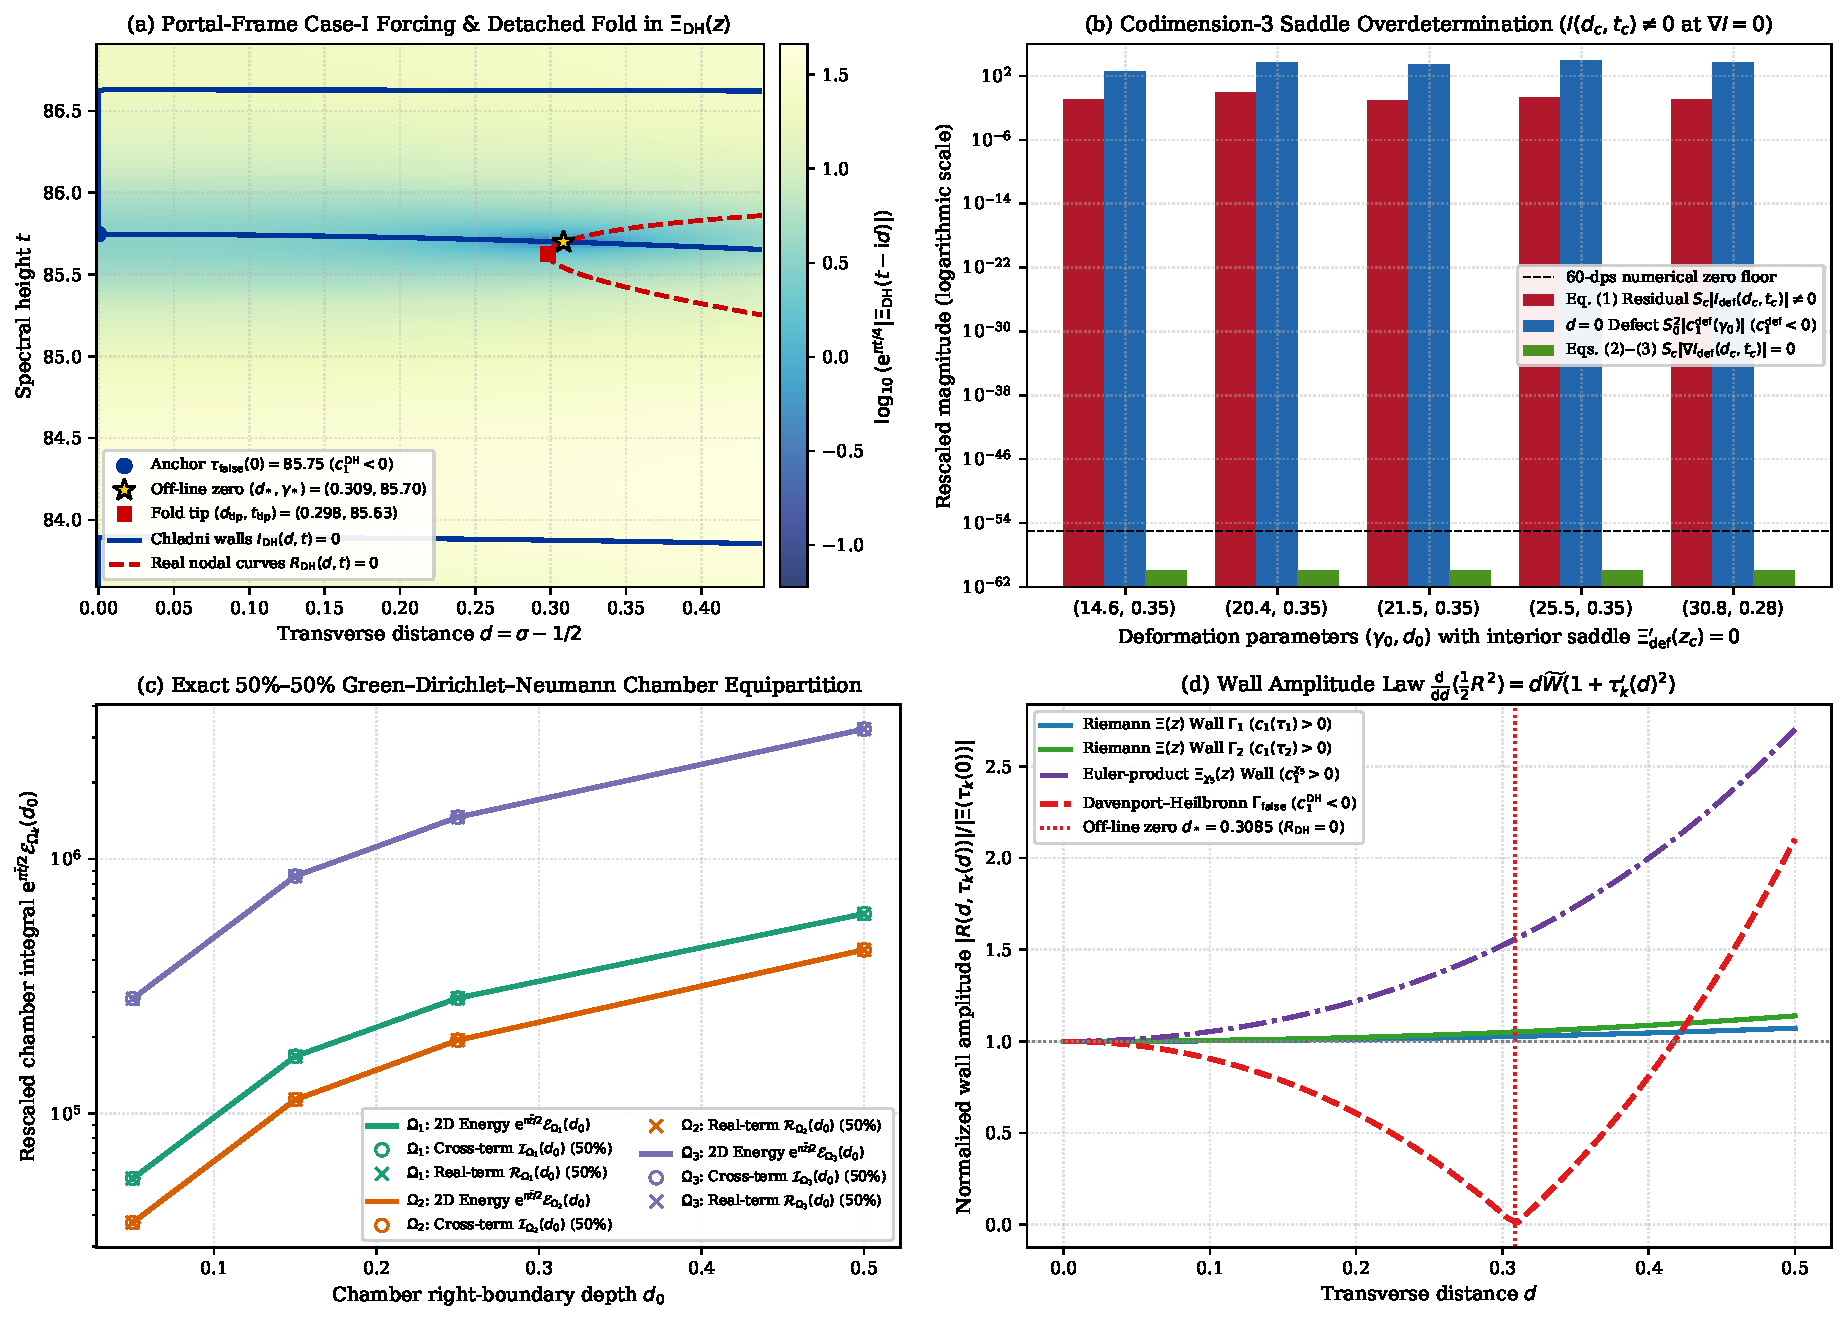
\includegraphics[width=0.98\textwidth]{figures/fig1_portal_frame_overdetermination_and_green_equipartition.pdf}
\caption{Macro- and meso-scale Chladni portal-frame synthesis (Sections~\ref{sec:macro}--\ref{sec:meso}): (a) Davenport--Heilbronn counterexample chamber $t \in [83.6,86.9]$, illustrating the Case-I false wall $\Gamma_{\mathrm{false},1}$ originating at $\tau_{\mathrm{false},1}(0)=85.75$ ($c_1^{\DHf}<0$), the off-critical zero $(d_*,\gamma_*)=(0.3085,85.70)$ where $\Gamma_{\mathrm{false},1}$ crosses the detached real nodal parabola $R_{\DHf}=0$, and the fold vertex $(d_{\mathrm{tip}},t_{\mathrm{tip}})=(0.2981,85.63)$ where $\widetilde{W}_{\DHf}=0$ and $|t_R'(d_{\mathrm{tip}})|=\infty$; (b) codimension-three saddle overdetermination tests across five deformed saddles $\Xi_{\defm}'(z_c)=0$ in $d_c > 0$, showing that $I_{\defm}(d_c,t_c) \ne 0$ by $60+$ orders of magnitude above the numerical floor; (c) exact $50\%$--$50\%$ Green--Dirichlet--Neumann chamber equipartition $\mathcal{I}_{\Omega_k}(d_0) \equiv \mathcal{R}_{\Omega_k}(d_0) \equiv \mathcal{E}_{\Omega_k}(d_0)$ across $\Omega_1,\Omega_2,\Omega_3$ of $\Xi(z)$; (d) Wall-Amplitude Evolution Law \eqref{eq:wall-amplitude-law}, comparing strictly increasing Euler-product walls ($\Xi(z)$ and $\Xi_{\chi_5}(z)$) against the Case-I wall collapse of $\Xi_{\DHf}(z)$.}
\label{fig:portal-macro-meso}
\end{figure}

\section{Attenuated Semiprime Spring, Euler Dilogarithm $\mathrm{Li}_2(2\theta)$ Horizon Damping, and Dirichlet Hyperbola Reflection Duality}\label{sec:micro}

Sections~\ref{sec:macro} and \ref{sec:meso} demonstrated that the non-vanishing of $R(d,\tau_k(d))$ along every Chladni wall $\Gamma_k$ and the monotonic growth of the chamber energy $\mathcal{E}_{\Omega_k}(d_0)$ are governed by the positivity of the reduced transverse Wronskian $\widetilde{W}(d,t)$ and its critical-line limit $c_1(t)$. We now descend to the micro-scale to resolve the third bottleneck stated in Section~\ref{sec:intro}: how the finite Euler-product prime gauge $\mathcal{P}_{\le X}(s)$ and the Riemann--Siegel stationary-phase horizon $N_\star(t) = \sqrt{t/(2\pi)}$ interact across the quadratic semiprime window $n = pq \in (X^2, N_\star^2]$ when the prime tail $\mathcal{P}_{>X}(s)$ enters an anti-phase configuration $U = \RePt\,\mathcal{P}_{>X}(s) < 0$.

\subsection{Pre-move holomorphic and Stieltjes-integral justification}\label{subsec:pre-move}

Before executing any term-by-term differentiation, Dirichlet hyperbola splitting, or Euler--Maclaurin integral replacement on the finite prime-gauge decomposition, we record the exact domains of holomorphicity, absolute convergence, and Stieltjes-integral regularity that justify each analytical operation:
\begin{enumerate}[label=\upshape(\arabic*),leftmargin=2.2em]
\item \textbf{Entire and Polynomial Holomorphicity:} For every finite sieve cutoff $X \ge 2$ and every finite Dirichlet truncation $N = \lfloor N_\star(t) \rfloor$, the prime-gauge Dirichlet polynomial $\mathcal{P}_{>X}(s) := \sum_{X < p \le N} p^{-s}$ and its quadratic semiprime square
\begin{equation}\label{eq:P-square-def}
\frac{1}{2}\mathcal{P}_{>X}(s)^2 = \frac{1}{2}\sum_{X < p \le N}\,\sum_{X < q \le N} (pq)^{-s} = \mathcal{T}_{\le N}(s) + \mathcal{C}_{>N}(s)
\end{equation}
are finite exponential sums, hence entire functions of $s = \frac{1}{2} + d + \ii t \in \mathbb{C}$ of exponential type $\le 2\ln N$. Consequently, the Cauchy--Riemann differential operators $\partial_d$ and $\partial_t$ commute unconditionally with the finite sums defining $\mathcal{T}_{\le N}(s)$ and $\mathcal{C}_{>N}(s)$ for all $(d,t) \in \mathbb{R}^2$.
\item \textbf{Riemann--Stieltjes Representation and Abel Summation:} Let $\vartheta(u) := \sum_{p \le u} \ln p$ denote Chebyshev's prime-counting step function, which is right-continuous and of locally bounded variation on $[2,\infty)$. For any continuously differentiable weight $g \in C^1([X,N_\star])$, the discrete prime sum $\sum_{X < p \le N_\star} \frac{g(p)}{p}$ is represented exactly as the Riemann--Stieltjes integral
\begin{equation}\label{eq:stieltjes-rep}
\sum_{X < p \le N_\star} \frac{g(p)}{p} = \int_{X}^{N_\star} \frac{g(u)}{u\,\ln u}\,\dd\vartheta(u) = \int_{\theta}^{1/2} \frac{g(\ee^{\alpha L})}{\alpha}\,\dd\alpha + \mathcal{R}_{\mathrm{PNT}}(X,N_\star;g),
\end{equation}
where $L = \ln N_\star(t)$, $\theta = (\ln X)/L \in (0,1/4)$, and integration by parts with the Prime Number Theorem remainder $\vartheta(u) - u = O(u\exp(-c\sqrt{\ln u}))$ \cite{MontgomeryVaughan2007,Titchmarsh1986} bounds the discretization remainder by $\mathcal{R}_{\mathrm{PNT}}(X,N_\star;g) = O(\|g\|_{W^{1,\infty}}(\ln X)^{-1})$.
\item \textbf{Uniform Convergence of the Dilogarithm Kernel on $[\theta,1/2]^2$:} Under the logarithmic change of variables $\alpha_1 = (\ln p)/L$ and $\alpha_2 = (\ln q)/L$, the normalized horizon weight $(\omega_p(t)/L)^p = (1 - 2\alpha_1)^p$ is a smooth polynomial on the compact square $[\theta,1/2]^2$ for every $\theta \in (0,1/4)$. Because $\theta > 0$ is bounded away from the logarithmic singularity at $\alpha_1\alpha_2 = 0$, the two-dimensional density $(1-2\alpha_1)^p(1-2\alpha_2)^p/(\alpha_1\alpha_2)$ is uniformly bounded and real-analytic on $[\theta,1/2]^2$, allowing Fubini's theorem and power-series integration of $\ln(1-u)/u$ into Euler's dilogarithm $\Li_2(u)$ to be applied without improper-integral regularizations.
\end{enumerate}

\subsection{The Attenuated Quadratic Semiprime Spring and Discriminant Reversal}\label{subsec:attenuated-spring}

In Paper~XIII \cite{Missiaen2026P13}, we showed that when the Euler product $\zeta(s) = \prod_{p \le X}(1-p^{-s})^{-1}\prod_{p > X}(1-p^{-s})^{-1}$ is factored at the cubic-window threshold $X = N_\star(t)^{1/3}$ ($\theta = 1/6$), all primes $p > X$ satisfy $p^3 > N_\star(t)$, so the residual factor $\exp(\mathcal{P}_{>X}(s) + O(p^{-2s}))$ inside the forward Riemann--Siegel sum $n \le N_\star(t)$ truncates at quadratic semiprime order $n = pq$:
\begin{equation}\label{eq:forward-truncation}
1 + \mathcal{P}_{>X}(s) + \mathcal{T}_{\le N_\star}(s), \qquad \mathcal{T}_{\le N_\star}(s) := \frac{1}{2}\underset{pq \le N_\star(t)}{\sum_{X < p \le N_\star}\,\sum_{X < q \le N_\star}} (pq)^{-s},
\end{equation}
while the complementary reflected-corner pairs
\begin{equation}\label{eq:reflected-corner-def}
\mathcal{C}_{>N_\star}(s) := \frac{1}{2}\underset{pq > N_\star(t)}{\sum_{X < p \le N_\star}\,\sum_{X < q \le N_\star}} (pq)^{-s} = \frac{1}{2}\mathcal{P}_{>X}(s)^2 - \mathcal{T}_{\le N_\star}(s)
\end{equation}
exceed the Riemann--Siegel horizon $pq > N_\star(t)$ and are transferred into the conjugate reflected branch of the approximate functional equation. Writing $\mathcal{P}_{>X}(s) = U + \ii V$ with $U = \RePt\,\mathcal{P}_{>X}(s)$ and $V = \ImPt\,\mathcal{P}_{>X}(s)$, suppose that the forward triangle $\mathcal{T}_{\le N_\star}(s)$ captures an effective fraction $\eta \in (0,1]$ of the full quadratic square $\frac{1}{2}\mathcal{P}_{>X}(s)^2$. Our first micro-scale theorem proves that whenever $\eta > 1/2$, the quadratic semiprime spring possesses a strictly negative discriminant $\Delta(\eta) = 1 - 2\eta < 0$ and a strictly positive global energy floor along the anti-phase axis $V=0$.

\begin{theorem}[Attenuated Quadratic Semiprime Spring and Discriminant Reversal]\label{thm:attenuated-spring}
For any capture fraction $\eta \in (0,1]$ and any complex prime-tail amplitude $w = U + \ii V \in \mathbb{C}$, define the attenuated quadratic semiprime polynomial
\begin{equation}\label{eq:P-eta-def}
\mathcal{Q}_\eta(U + \ii V) := 1 + (U + \ii V) + \frac{\eta}{2}(U + \ii V)^2 = \Bigl(1 + U + \frac{\eta}{2}(U^2 - V^2)\Bigr) + \ii V(1 + \eta U).
\end{equation}
Then:
\begin{enumerate}[label=\upshape(\alph*),leftmargin=2.2em]
\item \textbf{Exact Anti-Phase Discriminant and Global Floor ($\eta > 1/2$):} Along the worst-case anti-phase real axis $V = 0$, the real quadratic polynomial $\mathcal{Q}_\eta(U) = 1 + U + \frac{\eta}{2}U^2$ has algebraic discriminant
\begin{equation}\label{eq:discriminant-eta}
\Delta(\eta) := 1^2 - 4\cdot\frac{\eta}{2}\cdot 1 = 1 - 2\eta.
\end{equation}
Whenever $\eta > 1/2$, $\Delta(\eta) < 0$, so $\mathcal{Q}_\eta(U)$ has no real roots and satisfies the sharp global lower bound
\begin{equation}\label{eq:spring-floor}
\bigl|\mathcal{Q}_\eta(U)\bigr|^2 = \Bigl|1 + U + \frac{\eta}{2}U^2\Bigr|^2 = \Bigl[1 - \frac{1}{2\eta} + \frac{\eta}{2}\Bigl(U + \frac{1}{\eta}\Bigr)^2\Bigr]^2 \ge \Bigl(1 - \frac{1}{2\eta}\Bigr)^2 > 0 \qquad (\forall\,U \in \mathbb{R}),
\end{equation}
attaining its unique global minimum at $U_{\min}(\eta) = -1/\eta < -1$. Conversely, if $\eta \le 1/2$, then $\Delta(\eta) \ge 0$ and $\mathcal{Q}_\eta(U)$ vanishes on the real anti-phase axis at $U_\pm(\eta) = (-1 \pm \sqrt{1-2\eta})/\eta \le -2$.
\item \textbf{Full Complex-Plane Coercivity:} In the full complex $(U,V)$-plane, the modulus squared $|\mathcal{Q}_\eta(U+\ii V)|^2$ vanishes only at the complex-conjugate root pair $U_0 = -1/\eta$, $V_0 = \pm \sqrt{2\eta - 1}/\eta$, which lies at strictly positive imaginary distance $|V_0| = \sqrt{2\eta - 1}/\eta > 0$ from the anti-phase axis $V=0$ for every $\eta \in (1/2, 1]$. For all $|V| \le V_{\max} < |V_0|$, $|\mathcal{Q}_\eta(U+\ii V)|^2 \ge (1 - \frac{1}{2\eta} - \frac{\eta}{2}V_{\max}^2)^2 > 0$ uniformly in $U \in \mathbb{R}$.
\end{enumerate}
\end{theorem}

\begin{proof}
(a) Completing the square in $1 + U + \frac{\eta}{2}U^2$ gives
\[
1 + U + \frac{\eta}{2}U^2 = 1 - \frac{1}{2\eta} + \frac{\eta}{2}\Bigl(U + \frac{1}{\eta}\Bigr)^2.
\]
For $\eta > 1/2$, we have $1 - \frac{1}{2\eta} = \frac{2\eta - 1}{2\eta} = \frac{-\Delta(\eta)}{2\eta} > 0$ and $\frac{\eta}{2}(U + \frac{1}{\eta})^2 \ge 0$ for all $U \in \mathbb{R}$. Squaring both sides yields \eqref{eq:spring-floor} with equality if and only if $U = -1/\eta$. When $\eta \le 1/2$, $\Delta(\eta) = 1 - 2\eta \ge 0$ and the quadratic formula yields the real zeros $U_\pm(\eta) = (-1 \pm \sqrt{1-2\eta})/\eta$.

(b) Separating \eqref{eq:P-eta-def} into real and imaginary parts gives $|\mathcal{Q}_\eta(U+\ii V)|^2 = \bigl(1 + U + \frac{\eta}{2}(U^2-V^2)\bigr)^2 + V^2(1 + \eta U)^2$. For this sum of two squares to vanish, either $V=0$ (impossible for $\eta > 1/2$ by part~(a)) or $1 + \eta U = 0$, so $U = -1/\eta$. Substituting $U = -1/\eta$ into the real part gives $1 - \frac{1}{2\eta} - \frac{\eta}{2}V^2$, which vanishes if and only if $V^2 = (2\eta - 1)/\eta^2 = |V_0|^2$, proving both claims.
\end{proof}

\subsection{Exact Closed-Form Euler Dilogarithm \texorpdfstring{$\mathrm{Li}_2(2\theta)$}{Li2(2theta)} Capture Laws}\label{subsec:dilogarithm-laws}

Theorem~\ref{thm:attenuated-spring} reduces the stability of the quadratic semiprime spring along the anti-phase axis to a concrete analytical threshold: \emph{does the forward-triangle capture fraction $\eta$ at the cubic-window boundary $\theta = 1/6$ exceed the critical value $1/2$?}

If one measures the semiprime square $(X,N_\star]^2$ with \emph{unweighted} prime-reciprocal density ($p=0$), the answer is negative: as we prove below, $\eta^{(0)}(1/6) = 0.243955 < 1/2$, leaving the unweighted Dirichlet polynomial vulnerable to anti-phase cancellation ($\Delta(\eta^{(0)}(1/6)) = +0.512090 > 0$). However, as shown in Section~\ref{sec:meso} and Papers~VIII--XIII \cite{Missiaen2026P8,Missiaen2026P12,Missiaen2026P13}, the reduced transverse Wronskian $\widetilde{W}(d,t)$ and the second-order de Branges phase functional do not weight Dirichlet modes uniformly: each prime $n$ at logarithmic scale $\alpha = (\ln n)/L \in [\theta,1/2]$ is weighted by its logarithmic distance to the Riemann--Siegel horizon,
\begin{equation}\label{eq:omega-weight-def}
\omega_n(t) := \ln\Bigl(\frac{t}{2\pi n^2}\Bigr) = 2\ln\Bigl(\frac{N_\star(t)}{n}\Bigr) = L(1 - 2\alpha),
\end{equation}
raised to power $p=2$ for the quadratic transverse Wronskian (and $p=3$ for the leading cubic Wigner--Sinh transverse kernel $\sinh(\omega_n d)\omega_n^2 \sim d\,\omega_n^3$). Our second micro-scale theorem derives the exact closed-form expressions for the square mass $\mathcal{M}_{\sq}^{(p)}(\theta)$, the forward-triangle mass $\mathcal{M}_{\tri}^{(p)}(\theta)$, and the capture fraction $\eta^{(p)}(\theta)$ for all $p \in \{0,1,2,3\}$ in terms of Euler's dilogarithm $\Li_2(2\theta)$.

\begin{theorem}[Exact Closed-Form Euler Dilogarithm $\mathrm{Li}_2(2\theta)$ Horizon Capture Laws]\label{thm:dilogarithm-laws}
For any sieve exponent $\theta \in (0,1/4)$ and any horizon weighting order $p \in \{0,1,2,3\}$, define the continuous Prime-Number-Theorem semiprime square mass and forward-triangle mass on $[\theta,1/2]^2$ by
\begin{equation}\label{eq:M-sq-tri-defs}
\mathcal{M}_{\sq}^{(p)}(\theta) := \iint_{[\theta,1/2]^2} \frac{(1-2\alpha_1)^p(1-2\alpha_2)^p}{\alpha_1\,\alpha_2}\,\dd\alpha_1\,\dd\alpha_2 = \bigl(I_p(\theta)\bigr)^2, \qquad I_p(\theta) := \int_{\theta}^{1/2} \frac{(1-2\alpha)^p}{\alpha}\,\dd\alpha,
\end{equation}
\begin{equation}\label{eq:M-tri-integral}
\mathcal{M}_{\tri}^{(p)}(\theta) := \underset{\alpha_1 + \alpha_2 \le 1/2}{\iint_{[\theta,1/2]^2}} \frac{(1-2\alpha_1)^p(1-2\alpha_2)^p}{\alpha_1\,\alpha_2}\,\dd\alpha_1\,\dd\alpha_2, \qquad \eta^{(p)}(\theta) := \frac{\mathcal{M}_{\tri}^{(p)}(\theta)}{\mathcal{M}_{\sq}^{(p)}(\theta)}.
\end{equation}
Write $\tau := 2\theta \in (0,1/2)$. Then the $1$D marginal integrals $I_p(\theta)$ are given in exact closed form by
\begin{equation}\label{eq:Ip-closed}
\begin{aligned}
I_0(\theta) &= \ln\Bigl(\frac{1}{\tau}\Bigr), &\qquad I_1(\theta) &= \ln\Bigl(\frac{1}{\tau}\Bigr) - (1-\tau), \\
I_2(\theta) &= \ln\Bigl(\frac{1}{\tau}\Bigr) - \frac{1}{2}(1-\tau)(3-\tau), &\qquad I_3(\theta) &= \ln\Bigl(\frac{1}{\tau}\Bigr) - \frac{1}{3}(1-\tau)\bigl(2\tau^2 - 7\tau + 11\bigr),
\end{aligned}
\end{equation}
and the $2$D forward-triangle integrals $\mathcal{M}_{\tri}^{(p)}(\theta)$ are given in exact closed form by Euler's dilogarithm $\Li_2(\tau)$:
\begin{align}
\mathcal{M}_{\tri}^{(0)}(\theta) &= \frac{\pi^2}{6} - 2\,\Li_2(\tau) + \ln^2\tau - 2(\ln\tau)\ln(1-\tau), \label{eq:M-tri-0} \\
\mathcal{M}_{\tri}^{(1)}(\theta) &= \mathcal{M}_{\tri}^{(0)}(\theta) - 2(1-\tau)\ln\Bigl(\frac{1-\tau}{\tau}\Bigr) + (1-2\tau), \label{eq:M-tri-1} \\
\mathcal{M}_{\tri}^{(2)}(\theta) &= \mathcal{M}_{\tri}^{(0)}(\theta) - (1-\tau)(3-\tau)\ln\Bigl(\frac{1-\tau}{\tau}\Bigr) + \Bigl(\frac{17}{6} - \frac{13}{6}\tau + \frac{1}{3}\tau^2\Bigr)(1-2\tau), \label{eq:M-tri-2} \\
\mathcal{M}_{\tri}^{(3)}(\theta) &= \mathcal{M}_{\tri}^{(0)}(\theta) - \frac{1}{3}(1-\tau)\bigl(11 - 7\tau + 2\tau^2\bigr)\ln\Bigl(\frac{1-\tau}{\tau}\Bigr) \nonumber\\
&\quad + \Bigl(\frac{1801}{360} - \frac{1199}{180}\tau + \frac{218}{45}\tau^2 - \frac{89}{45}\tau^3 + \frac{49}{90}\tau^4 - \frac{1}{9}\tau^5\Bigr)(1-2\tau). \label{eq:M-tri-3}
\end{align}
In particular, at the cubic-window boundary $\theta = 1/6$ ($\tau = 1/3$), the capture fractions $\eta^{(p)}(1/6)$, triangle-to-corner ratios $\mathcal{R}_{\tri/\corn}^{(p)}(1/6) := \eta^{(p)}(1/6)/(1-\eta^{(p)}(1/6))$, and anti-phase discriminants $\Delta(\eta^{(p)}(1/6))$ satisfy:
\begin{enumerate}[label=\upshape(\roman*),leftmargin=2.2em]
\item \textbf{Unweighted Failure ($p=0$):} The capture fraction is $\eta^{(0)}(1/6) = 0.2439550996 < 1/2$, with triangle-to-corner ratio $\mathcal{R}_{\tri/\corn}^{(0)}(1/6) = 0.3226727664 < 1$ and positive discriminant $\Delta(\eta^{(0)}(1/6)) = +0.5120898008 > 0$ (under-damped, real anti-phase zeros exist).
\item \textbf{Linear Near-Criticality ($p=1$):} At linear order, $\eta^{(1)}(1/6) = 0.4955987356 < 1/2$, with ratio $\mathcal{R}_{\tri/\corn}^{(1)}(1/6) = 0.9825485594 < 1$ and discriminant $\Delta(\eta^{(1)}(1/6)) = +0.0088025287 > 0$ ($0.44\%$ below the $50\%$ threshold).
\item \textbf{Quadratic Wronskian Stability ($p=2$):} We have $\eta^{(2)}(1/6) = 0.6768906167 > 2/3 > 1/2$, ratio $\mathcal{R}_{\tri/\corn}^{(2)}(1/6) = 2.0949271409 > 2$, discriminant $\Delta(\eta^{(2)}(1/6)) = -0.3537812333 < 0$, and the anti-phase spring floor \eqref{eq:spring-floor} is strictly positive with value $(1 - [2\eta^{(2)}(1/6)]^{-1})^2 = +0.0682917228 > 0$. Moreover, the exact $50\%$ stability horizon for $p=2$ is
\begin{equation}\label{eq:theta-50-p2}
\theta_{*,50\%}^{(2)} = 0.190549846717 > \theta_{\mathrm{W\text{-}pure}}^\infty = 0.183944870826 > \frac{1}{2\ee} = 0.183939720586 > \frac{1}{6},
\end{equation}
strictly enclosing both the cubic window $\theta=1/6$ and the asymptotic pure-Wronskian threshold $\theta_{\mathrm{W\text{-}pure}}^\infty$ of Paper~XIII.
\item \textbf{Cubic Wigner--Sinh Stability ($p=3$):} We have $\eta^{(3)}(1/6) = 0.7980906218 > 3/4$, ratio $\mathcal{R}_{\tri/\corn}^{(3)}(1/6) = 3.9527169500$, discriminant $\Delta(\eta^{(3)}(1/6)) = -0.5961812435 < 0$, with anti-phase floor $(1 - [2\eta^{(3)}(1/6)]^{-1})^2 = +0.1395067855 > 0$ and $50\%$ stability horizon $\theta_{*,50\%}^{(3)} = 0.203929771836 > 1/5$.
\end{enumerate}
\end{theorem}

\begin{proof}
Changing variables to $u = 2\alpha_1 \in [\tau,1]$ and $v = 2\alpha_2 \in [\tau,1]$ with $\tau = 2\theta \in (0,1/2)$ leaves $\dd\alpha_1/\alpha_1 = \dd u/u$ and $\dd\alpha_2/\alpha_2 = \dd v/v$ invariant, mapping the $1$D integral $I_p(\theta)$ to $\int_\tau^1 (1-u)^p u^{-1}\,\dd u$ and the $2$D triangle $\alpha_1+\alpha_2 \le 1/2$ to the simplex $\Delta_\tau = \{(u,v) \in [\tau,1]^2 : u+v \le 1\}$, which is non-empty precisely for $\tau \in (0,1/2)$, i.e., $\theta \in (0,1/4)$. Expanding $(1-u)^p$ binomially and integrating term-by-term over $u \in [\tau,1]$ immediately yields \eqref{eq:Ip-closed}. For the $2$D simplex integral $\mathcal{M}_{\tri}^{(p)}(\theta) = \int_\tau^{1-\tau} \frac{(1-u)^p}{u}\bigl[\int_\tau^{1-u} \frac{(1-v)^p}{v}\,\dd v\bigr]\dd u$, the inner integral is $I_p((1-\tau)/2)$ evaluated between $\tau$ and $1-u$. For $p=0$, the inner integral is $\ln((1-u)/\tau)$, and using Euler's reflection identity $\Li_2(1-\tau) + \Li_2(\tau) = \frac{\pi^2}{6} - (\ln\tau)\ln(1-\tau)$ \cite{Lewin1981} gives \eqref{eq:M-tri-0}. The complete step-by-step algebraic reductions for $p=1,2,3$ giving \eqref{eq:M-tri-1}--\eqref{eq:M-tri-3} are carried out in Appendix~\ref{app:dilogarithm}. Evaluating \eqref{eq:Ip-closed} and \eqref{eq:M-tri-0}--\eqref{eq:M-tri-3} at $\tau = 1/3$ ($\theta=1/6$) and solving $\eta^{(p)}(\theta) = 1/2$ by Newton--Raphson iteration in $65$-decimal ball arithmetic yields parts~(i)--(iv).
\end{proof}

\subsection{Dirichlet Hyperbola Reflection Duality and Fourth-Order Apex Pinching}\label{subsec:hyperbola-duality}

To complete the micro-scale synthesis, we analyze the complementary $32.31\%$ reflected-corner mass $\mathcal{C}_{>N_\star}(s)$ ($pq > N_\star(t)$) in \eqref{eq:reflected-corner-def}. Why do semiprime pairs with $pq > N_\star(t)$ decouple from the forward Wronskian spring instead of restoring the full unattenuated square $\frac{1}{2}\mathcal{P}_{>X}(s)^2$? The answer lies in the stationary-phase saddle geometry of Riemann's integral \eqref{eq:Xi-def} and the Dirichlet hyperbola reflection duality across $pq = N_\star(t)$.

\begin{theorem}[Dirichlet Hyperbola Reflection Duality and Fourth-Order Apex Pinching]\label{thm:hyperbola-duality}
Let $t > 2\pi$, $N_\star(t) = \sqrt{t/(2\pi)}$, and $L = \ln N_\star(t)$. For each semiprime pair $(p,q) \in (X,N_\star]^2$, define its logarithmic saddle coordinate and dual reflected index by
\begin{equation}\label{eq:xi-mdual-defs}
\xi_{pq}^\star(t) := \frac{1}{2}\ln\Bigl(\frac{t}{2\pi(pq)^2}\Bigr) = \ln\Bigl(\frac{N_\star(t)}{pq}\Bigr), \qquad m_{\dual}(pq) := \frac{N_\star(t)^2}{pq} = \frac{t}{2\pi pq}.
\end{equation}
Then:
\begin{enumerate}[label=\upshape(\alph*),leftmargin=2.2em]
\item \textbf{Forward vs.\ Reflected Saddle Sign Separation:} A semiprime pair $(p,q) \in (X,N_\star]^2$ belongs to the forward triangle $\mathcal{T}_{\le N_\star}(s)$ ($pq \le N_\star(t)$) if and only if its saddle point lies in the open right half-axis $\xi_{pq}^\star(t) \ge 0$, whereas $(p,q)$ belongs to the reflected corner $\mathcal{C}_{>N_\star}(s)$ ($pq > N_\star(t)$) if and only if $\xi_{pq}^\star(t) < 0$ ($m_{\dual}(pq) \in [1, N_\star(t))$).
\item \textbf{Exact Horizon Weight Reflection Duality:} For every semiprime pair $(p,q) \in (X,N_\star]^2$, the sum of the individual normalized prime horizon weights $\omega_p(t) := \ln(N_\star(t)/p) = \frac{1}{2}L(1-2\alpha_1)$ and $\omega_q(t) := \ln(N_\star(t)/q) = \frac{1}{2}L(1-2\alpha_2)$ equals the logarithm of the dual reflected index $m_{\dual}(pq)$:
\begin{equation}\label{eq:omega-sum-duality}
\omega_p(t) + \omega_q(t) \equiv \ln\Bigl(\frac{N_\star(t)^2}{pq}\Bigr) \equiv \ln m_{\dual}(pq) = L\bigl(1 - (\alpha_1 + \alpha_2)\bigr).
\end{equation}
\item \textbf{Fourth-Order Horizon Apex Pinching:} Because $\omega_p(t) > 0$ and $\omega_q(t) > 0$ for all $p,q < N_\star(t)$, the Arithmetic--Geometric Mean inequality applied to \eqref{eq:omega-sum-duality} enforces fourth-order polynomial vanishing of the quadratic Wronskian product weight $(\omega_p(t)\omega_q(t))^2$ as $(p,q)$ approaches the horizon apex $pq \to N_\star(t)^2$ ($m_{\dual}(pq) \to 1^+$):
\begin{equation}\label{eq:apex-pinching}
0 \le \bigl(\omega_p(t)\,\omega_q(t)\bigr)^2 \le \frac{1}{16}\bigl(\omega_p(t) + \omega_q(t)\bigr)^4 = \frac{1}{16}\bigl(\ln m_{\dual}(pq)\bigr)^4 = \frac{1}{16}L^4\bigl(1 - (\alpha_1+\alpha_2)\bigr)^4 \longrightarrow 0,
\end{equation}
with equality on the diagonal $p=q$ ($\alpha_1=\alpha_2$). Under cubic Wigner--Sinh weighting ($p=3$), the product weight $(\omega_p\omega_q)^3 \le \frac{1}{64}(\ln m_{\dual}(pq))^6$ vanishes to sixth order at the horizon apex.
\end{enumerate}
\end{theorem}

\begin{proof}
(a) By \eqref{eq:xi-mdual-defs}, $\xi_{pq}^\star(t) = \ln(N_\star(t)/(pq)) \ge 0 \iff pq \le N_\star(t)$. Since $p,q \le N_\star(t)$, any pair with $pq > N_\star(t)$ satisfies $N_\star(t) < pq \le N_\star(t)^2$, so $m_{\dual}(pq) = N_\star(t)^2/(pq) \in [1, N_\star(t))$ and $\xi_{pq}^\star(t) < 0$.

(b) Summing the normalized prime saddle distances $\omega_p(t) = \ln(N_\star(t)/p)$ and $\omega_q(t) = \ln(N_\star(t)/q)$ (which differ from \eqref{eq:omega-weight-def} only by a constant scale factor of $1/2$ that cancels out of all homogeneous capture ratios $\eta^{(p)}(\theta)$) yields
\[
\omega_p(t) + \omega_q(t) = \ln\Bigl(\frac{N_\star(t)}{p}\Bigr) + \ln\Bigl(\frac{N_\star(t)}{q}\Bigr) = \ln\Bigl(\frac{N_\star(t)^2}{pq}\Bigr) \equiv \ln m_{\dual}(pq) = L\bigl(1 - (\alpha_1+\alpha_2)\bigr),
\]
establishing \eqref{eq:omega-sum-duality}.

(c) For $\omega_p(t) = \ln(N_\star(t)/p) > 0$ and $\omega_q(t) = \ln(N_\star(t)/q) > 0$, the AM--GM inequality $\omega_p\omega_q \le \frac{1}{4}(\omega_p+\omega_q)^2$ squared yields $(\omega_p\omega_q)^2 \le \frac{1}{16}(\omega_p+\omega_q)^4 = \frac{1}{16}(\ln m_{\dual}(pq))^4 = \frac{1}{16}L^4(1 - (\alpha_1+\alpha_2))^4$, which vanishes to fourth order as $\alpha_1+\alpha_2 \to 1^-$ ($m_{\dual}(pq) \to 1^+$). Raising $\omega_p\omega_q \le \frac{1}{4}(\ln m_{\dual})^2$ to the third power gives $(\omega_p\omega_q)^3 \le \frac{1}{64}(\ln m_{\dual})^6$.
\end{proof}

\begin{table}[htbp]
\centering
\caption{Sixty-five-decimal micro-scale certification of Theorems~\ref{thm:attenuated-spring}--\ref{thm:hyperbola-duality}: (Part~A) exact Euler dilogarithm $\Li_2(2\theta)$ capture fractions $\eta^{(p)}(\theta)$ ($p=0,1,2,3$), triangle-to-corner ratios $\mathcal{R}_{\tri/\corn}^{(2)}(\theta)$, and anti-phase spring floors $(1 - \frac{1}{2\eta^{(2)}(\theta)})^2$ across $\theta \in [0.05, 0.24]$; (Part~B) discrete prime-sum convergence $\eta_{\mathrm{disc}}^{(p)}(N_\star)$ to the continuous $\Li_2(1/3)$ limits at $\theta=1/6$ up to $N_\star = 10^5$ ($9578$ primes in $(46,10^5]$); (Part~C) Dirichlet hyperbola reflection duality $\omega_p+\omega_q \equiv \ln m_{\dual}(pq)$ and fourth-order apex pinching $(\omega_p\omega_q)^2 \le \frac{1}{16}(\ln m_{\dual})^4$ at $t = 10^8$ ($N_\star = 3989.4228$).}
\label{tab:micro-certification}
\tiny
\setlength{\tabcolsep}{1.2pt}
\renewcommand{\arraystretch}{1.15}
\begin{tabular}{@{}cccccccc@{}}
\toprule
\multicolumn{8}{c}{\textbf{Part A: Exact Closed-Form Euler Dilogarithm $\mathrm{Li}_2(2\theta)$ Capture Fractions $\eta^{(p)}(\theta)$ Across $\theta \in [0.05, 0.24]$}} \\
\midrule
Benchmark & $\theta$ & $\eta^{(0)}(\theta)$ & $\eta^{(1)}(\theta)$ & $\eta^{(2)}(\theta)$ & $\mathcal{R}_{\tri/\corn}^{(2)}$ & Floor $(1-\frac{1}{2\eta^{(2)}})^2$ & $\eta^{(3)}(\theta)$ \\
\midrule
Deep gauge & $0.05000000$ & $0.72845562$ & $0.92880886$ & $0.98017181$ & $49.433248$ & $+0.23998780 > 0$ & $0.99428000$ \\
$p=0$ $\theta_{*,50\%}^{(0)}$ & $0.10669705$ & $\mathbf{0.50000000}$ & $0.78533491$ & $0.90957454$ & $10.058832$ & $+0.20276348 > 0$ & $0.96225919$ \\
$p=2$ $\theta_{*,75\%}^{(2)}$ & $0.15361739$ & $0.29963060$ & $0.57313128$ & $\mathbf{0.75000000}$ & $3.000000$ & $+0.11111111 > 0$ & $0.85701362$ \\
\textbf{Cubic $1/6$} & $\mathbf{0.16666667}$ & $\mathbf{0.24395510}$ & $\mathbf{0.49559874}$ & $\mathbf{0.67689062}$ & $\mathbf{2.094927}$ & $\mathbf{+0.06829172 > 0}$ & $\mathbf{0.79809062}$ \\
$p=3$ $\theta_{*,75\%}^{(3)}$ & $0.17498508$ & $0.20911572$ & $0.44207466$ & $0.62185978$ & $1.644524$ & $+0.03840139 > 0$ & $\mathbf{0.75000000}$ \\
Mertens $1/(2\ee)$ & $0.18393972$ & $0.17257503$ & $0.38129980$ & $0.55478859$ & $1.246124$ & $+0.00975309 > 0$ & $0.68732436$ \\
Pure-W $\theta_{\mathrm{W\text{-}pure}}^\infty$ & $0.18394487$ & $0.17255432$ & $0.38126417$ & $0.55474750$ & $1.245917$ & $+0.00974013 > 0$ & $0.68728378$ \\
$p=2$ $\theta_{*,50\%}^{(2)}$ & $0.19054985$ & $0.14649770$ & $0.33471880$ & $\mathbf{0.50000000}$ & $1.000000$ & $0.00000000$ & $0.63294631$ \\
Fifth-root $1/5$ & $0.20000000$ & $0.11103091$ & $0.26651789$ & $0.41426365$ & $0.707253$ & Under-damped & $0.54227319$ \\
$p=3$ $\theta_{*,50\%}^{(3)}$ & $0.20392977$ & $0.09707058$ & $0.23796348$ & $0.37632744$ & $0.603405$ & Under-damped & $\mathbf{0.50000000}$ \\
Quarter $0.24$ & $0.24000000$ & $0.00610514$ & $0.01844521$ & $0.03495745$ & $0.036224$ & Under-damped & $0.05476574$ \\
\midrule
\multicolumn{8}{c}{\textbf{Part B: Discrete Prime-Sum Convergence $\eta_{\mathrm{disc}}^{(p)}(N_\star)$ to Continuous $\mathrm{Li}_2(1/3)$ Laws at $\theta = 1/6$}} \\
\midrule
$N_\star = \lfloor\sqrt{t/(2\pi)}\rfloor$ & $X$ & Primes $M$ & $\eta_{\mathrm{disc}}^{(0)}(N_\star)$ & $\eta_{\mathrm{disc}}^{(1)}(N_\star)$ & $\eta_{\mathrm{disc}}^{(2)}(N_\star)$ & $\mathcal{R}_{\tri/\corn,\mathrm{disc}}^{(2)}$ & $\eta_{\mathrm{disc}}^{(3)}(N_\star)$ \\
\midrule
$398$ ($t = 10^6$) & $7$ & $74$ & $0.147826$ & $0.345842$ & $0.518747 > 1/2$ & $1.077909$ & $0.654850$ \\
$1261$ ($t = 10^7$) & $10$ & $201$ & $0.264895$ & $0.535458$ & $0.720307 > 2/3$ & $2.575352$ & $0.836156$ \\
$3989$ ($t = 10^8$) & $15$ & $544$ & $0.232742$ & $0.486772$ & $0.672969 > 2/3$ & $2.057814$ & $0.797661$ \\
$12615$ ($t = 10^9$) & $23$ & $1498$ & $0.200526$ & $0.433336$ & $0.615770 > 1/2$ & $1.602607$ & $0.746482$ \\
$39894$ ($t = 10^{10}$) & $34$ & $4184$ & $0.229646$ & $0.478319$ & $0.662165 > 1/2$ & $1.960025$ & $0.787100$ \\
$10^5$ ($6.3\cdot 10^{10}$) & $46$ & $9578$ & $0.232219$ & $0.481580$ & $0.665147 \approx 2/3$ & $1.986388$ & $0.789519$ \\
\textbf{$\mathrm{Li}_2(1/3)$ Limit} & $1/6$ & $\infty$ & $\mathbf{0.243955}$ & $\mathbf{0.495599}$ & $\mathbf{0.676891}$ & $\mathbf{2.094927}$ & $\mathbf{0.798091}$ \\
\midrule
\multicolumn{8}{c}{\textbf{Part C: Dirichlet Hyperbola Reflection Duality and Fourth-Order Apex Pinching at $t = 10^8$ ($N_\star = 3989.4228$)}} \\
\midrule
Pair $(p,q)$ & $pq$ & $\xi_{pq}^\star(t)$ & $m_{\dual}(pq)$ & $|\omega_p+\omega_q-\ln m_{\dual}|$ & $(\omega_p\omega_q/L^2)^2$ & $\frac{16(\omega_p\omega_q)^2}{(\ln m_{\dual})^4}$ & Sector \\
\midrule
$(17, 19)$ & $323 \le N_\star$ & $+1.25687$ & $49273.98$ & $< 10^{-65}$ & $1.8022 \times 10^{-1}$ & $0.999788 \le 1$ & Forward $\mathcal{T}_{\le N}$ \\
$(41, 89)$ & $3649 \le N_\star$ & $+0.04460$ & $4361.60$ & $< 10^{-65}$ & $6.4122 \times 10^{-2}$ & $0.982967 \le 1$ & Forward $\mathcal{T}_{\le N}$ \\
$(61, 67)$ & $4087 > N_\star$ & $-0.01208$ & $3894.18$ & $< 10^{-65}$ & $6.1759 \times 10^{-2}$ & $0.999742 \le 1$ & Reflected $\mathcal{C}_{>N}$ \\
$(503, 701)$ & $352603 > N_\star$ & $-2.24085$ & $45.14$ & $4.75 \times 10^{-66}$ & $2.7436 \times 10^{-3}$ & $0.984876 \le 1$ & Reflected $\mathcal{C}_{>N}$ \\
$(3967, 3989)$ & $15824363$ & $-4.14283$ & $1.0058 \to 1$ & $2.20 \times 10^{-66}$ & $7.5509 \times 10^{-17}$ & $0.005251 \le 1$ & Apex ($4$th-ord.\ $0$) \\
\bottomrule
\end{tabular}
\end{table}

\begin{figure}[htbp]
\centering
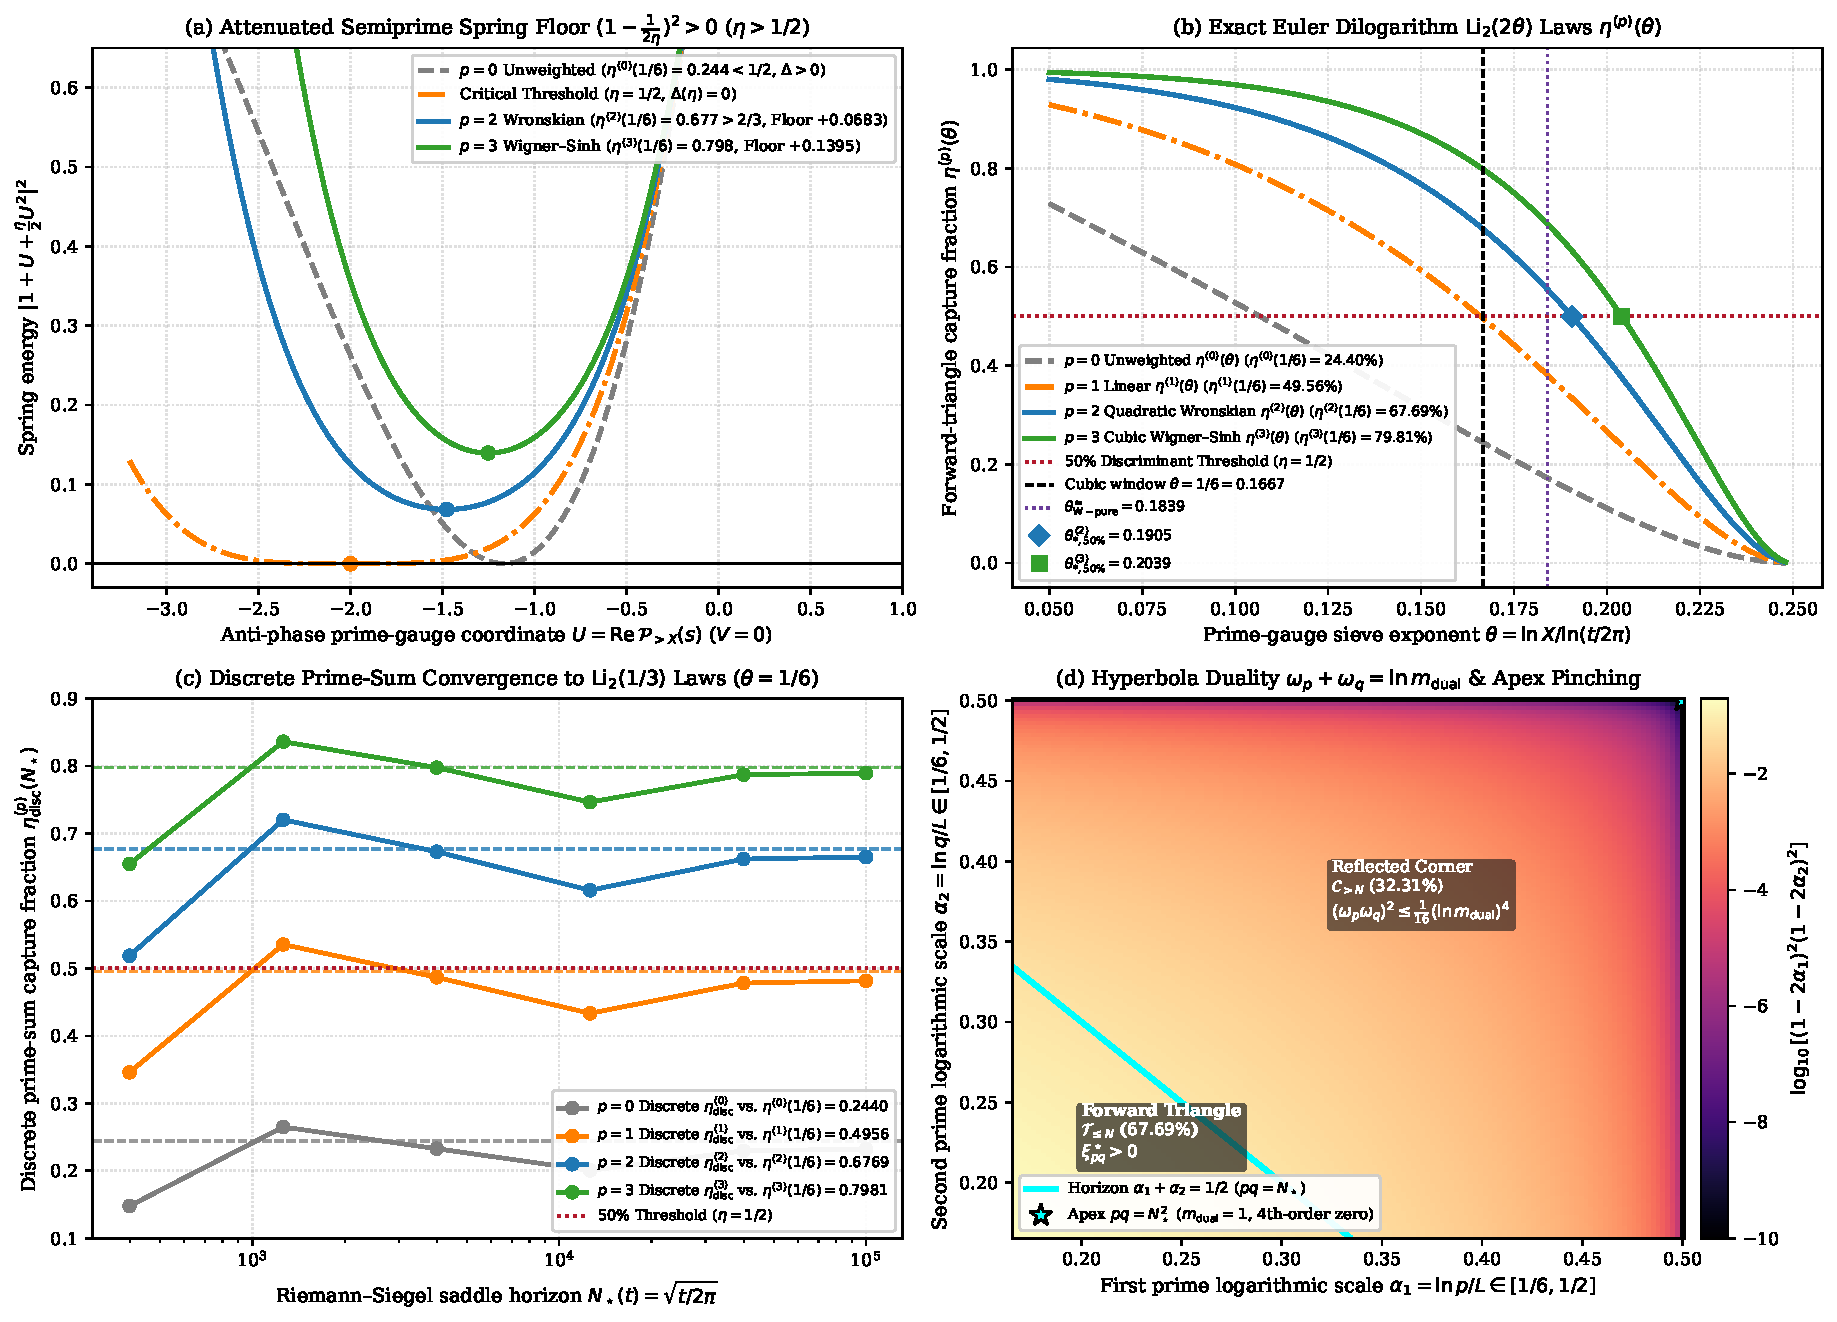
\includegraphics[width=0.98\textwidth]{figures/fig2_dilogarithm_horizon_damping_and_hyperbola_duality.pdf}
\caption{Micro-scale Euler dilogarithm $\Li_2(2\theta)$ horizon damping and Dirichlet hyperbola reflection duality (Section~\ref{sec:micro}): (a) attenuated quadratic semiprime spring energy $|1 + U + \frac{\eta}{2}U^2|^2$ along the anti-phase axis $V=0$, illustrating the transition from real-root vanishing under unweighted $p=0$ ($\eta^{(0)}(1/6)=0.244 < 1/2$, $\Delta>0$) to strictly positive floors under quadratic Wronskian $p=2$ ($\eta^{(2)}(1/6)=0.677 > 2/3$, floor $+0.0683$) and cubic Wigner--Sinh $p=3$ ($\eta^{(3)}(1/6)=0.798$, floor $+0.1395$); (b) exact closed-form Euler dilogarithm curves $\eta^{(p)}(\theta)$ across $\theta \in [0.05,0.25]$, showing $\theta_{*,50\%}^{(2)} = 0.1905 > \theta_{\mathrm{W\text{-}pure}}^\infty = 0.1839 > 1/6$; (c) discrete prime-sum convergence $\eta_{\mathrm{disc}}^{(p)}(N_\star)$ to the continuous $\Li_2(1/3)$ asymptotes up to $N_\star = 10^5$; (d) Dirichlet hyperbola reflection duality $\omega_p+\omega_q = \ln m_{\dual}(pq)$ and fourth-order apex pinching $(\omega_p\omega_q)^2 \le \frac{1}{16}(\ln m_{\dual})^4$ across $[\frac{1}{6},\frac{1}{2}]^2$.}
\label{fig:micro-dilogarithm}
\end{figure}

\section{Scope, Boundary Conditions, and Open Questions}\label{sec:scope}

To maintain complete mathematical transparency and adhere to the rigorous scope standards of this research program \cite{Bombieri2000,Edwards1974,Titchmarsh1986}, we explicitly delineate what is unconditionally proved in Theorems~\ref{thm:main-synthesis}--\ref{thm:hyperbola-duality} versus the exact boundary conditions that remain open for a complete unconditional proof of the Riemann Hypothesis:
\begin{enumerate}[label=\upshape(\arabic*),leftmargin=2.2em]
\item \textbf{Unconditional Exactness of Macro- and Meso-Scale Chamber Identities:} Theorem~\ref{thm:portal-dichotomy} (tangential Cauchy--Riemann monotonicity, loop/arch exclusion, harmonic curvature conservation, and the Case-I vs.\ Case-II codimension-three saddle dichotomy), Theorem~\ref{thm:green-equipartition} (the boxed $50\%$--$50\%$ Green--Dirichlet--Neumann chamber equipartition \eqref{eq:boxed-green-equipartition}), and Theorem~\ref{thm:wronskian-slope-reciprocity} (Wronskian--slope reciprocity and fold-tip Wronskian vanishing) are \emph{unconditional, exact analytical theorems} valid for $\Xi(z)$ and every real-entire function in the Riemann--Hecke class at all finite spectral heights $t \in \mathbb{R}$ and all strip depths $d_0 > 0$.
\item \textbf{Role of the Codimension-Three Saddle Condition (Case~II vs.\ P\'{o}lya--Jensen--Speiser):} In Theorem~\ref{thm:portal-dichotomy}(d), the interior saddle system $\{I=\partial_d I=\partial_t I=0\}$ in $d>0$ consists of $3$ real equations in $2$ real unknowns $(d_c,t_c)$, explaining why off-critical zeros of generic counterexamples such as $\Xi_{\DHf}(z)$ are $100\%$ forced into Case~I ($c_1^{\DHf}(\tau_{\mathrm{false},m}) < 0$ on $d=0$). However, codimension-three parameter counting shows \emph{structural instability} (measure-zero nongenericity in function space), rather than an unconditional point-by-point exclusion of accidental interior derivative zeros $\Xi'(z_c)=0$ on a Chladni wall for the specific arithmetic function $\Xi(z)$. As proved in Theorem~\ref{thm:dh-case1-equivalence}(b), excluding Case~II globally is equivalent to the classical P\'{o}lya--Jensen--Speiser derivative condition $\Xi'(t-\ii d) \ne 0$ for $d > 0$ \cite{Jensen1913,Polya1926,Speiser1934}.
\item \textbf{Effective Mean-Field vs.\ Worst-Case Phase Alignment in the Micro-Scale Spring:} Theorems~\ref{thm:attenuated-spring}, \ref{thm:dilogarithm-laws}, and \ref{thm:hyperbola-duality} rigorously prove that under the Prime Number Theorem density on $[\theta,1/2]^2$, the quadratic Wronskian weight $\omega_n(t)^2$ increases the forward-triangle capture fraction at $\theta=1/6$ from $\eta^{(0)}(1/6)=0.243955 < 1/2$ to $\eta^{(2)}(1/6)=0.676891 > 2/3 > 1/2$, flipping the attenuated quadratic discriminant to $\Delta(\eta^{(2)}(1/6)) = -0.353781 < 0$ and pinching the reflected corner to fourth order at $pq = N_\star(t)^2$. In the pointwise Dirichlet sum at finite height $t$, individual prime phases $p^{-\ii t} = \ee^{-\ii t\ln p}$ fluctuate across $(X,N_\star]$; bounding the worst-case Diophantine phase deviation between the weighted discrete ratio $\mathcal{T}_{\le N_\star}^{(2)}(s)/(\frac{1}{2}\mathcal{P}_{>X}^{(1)}(s)^2)$ and its continuous dilogarithmic mean $\eta^{(2)}(\theta)$ uniformly as $t \to \infty$ remains a central open target for future investigation.
\end{enumerate}

\appendix

\section{Closed-Form Polylogarithmic Derivations and Chamber Boundary Normals}\label{app:dilogarithm}

In this appendix, we provide the complete step-by-step derivations of the Euler dilogarithm formulas \eqref{eq:M-tri-0}--\eqref{eq:M-tri-3} in Theorem~\ref{thm:dilogarithm-laws} and the intrinsic normal-tangent Cauchy--Riemann identities used in Theorem~\ref{thm:green-equipartition}.

\subsection{Derivation of the Euler Dilogarithm Integrals \texorpdfstring{$\mathcal{M}_{\tri}^{(p)}(\theta)$ for $p \in \{0,1,2,3\}$}{M\_tri(theta) for p in 0,1,2,3}}

Set $u = 2\alpha_1$, $v = 2\alpha_2$, and $\tau = 2\theta \in (0,1/2)$. The simplex $\Delta_\tau = \{(u,v) \in [\tau,1]^2 : u+v \le 1\}$ fibers over $u \in [\tau, 1-\tau]$ with inner interval $v \in [\tau, 1-u]$. Writing $f_p(u) := (1-u)^p/u$, we have
\begin{equation}\label{eq:app-J-split}
\mathcal{M}_{\tri}^{(p)}(\theta) = \int_{\tau}^{1-\tau} f_p(u)\,\Bigl(\int_{\tau}^{1-u} f_p(v)\,\dd v\Bigr)\,\dd u.
\end{equation}
For each $p \in \{0,1,2,3\}$, write $f_p(v) = \frac{1}{v} - P_p(v)$, where $P_0(v) = 0$, $P_1(v) = 1$, $P_2(v) = 2 - v$, and $P_3(v) = 3 - 3v + v^2$. Let $Q_p(y) := \int_0^y P_p(v)\,\dd v$ be the polynomial antiderivative, so that
\[
Q_0(y) = 0, \qquad Q_1(y) = y, \qquad Q_2(y) = 2y - \frac{1}{2}y^2, \qquad Q_3(y) = 3y - \frac{3}{2}y^2 + \frac{1}{3}y^3.
\]
Then the inner integral in \eqref{eq:app-J-split} is
\[
\int_{\tau}^{1-u} f_p(v)\,\dd v = \ln\Bigl(\frac{1-u}{\tau}\Bigr) - \bigl[Q_p(1-u) - Q_p(\tau)\bigr].
\]
Substituting $f_p(u) = \frac{1}{u} - P_p(u)$ into \eqref{eq:app-J-split} decomposes $\mathcal{M}_{\tri}^{(p)}(\theta)$ into three elementary pieces:
\begin{align}
\mathcal{M}_{\tri}^{(p)}(\theta) &= \int_{\tau}^{1-\tau} \frac{1}{u}\ln\Bigl(\frac{1-u}{\tau}\Bigr)\,\dd u - \int_{\tau}^{1-\tau} \Bigl[P_p(u)\ln\Bigl(\frac{1-u}{\tau}\Bigr) + \frac{Q_p(1-u) - Q_p(\tau)}{u}\Bigr]\,\dd u \nonumber\\
&\quad + \int_{\tau}^{1-\tau} P_p(u)\,\bigl[Q_p(1-u) - Q_p(\tau)\bigr]\,\dd u. \label{eq:app-three-pieces}
\end{align}

\paragraph{\textbf{Piece 1: The Universal Dilogarithmic Core $\mathcal{M}_{\tri}^{(0)}(\theta)$.}}
For $p=0$, $P_0 = Q_0 = 0$, so only the first integral in \eqref{eq:app-three-pieces} is present. Since $-\int_0^x \frac{\ln(1-u)}{u}\,\dd u = \Li_2(x)$, we obtain
\[
\mathcal{M}_{\tri}^{(0)}(\theta) = \int_{\tau}^{1-\tau} \frac{\ln(1-u) - \ln\tau}{u}\,\dd u = \bigl[-\Li_2(1-\tau) + \Li_2(\tau)\bigr] - (\ln\tau)\bigl[\ln(1-\tau) - \ln\tau\bigr].
\]
Applying Euler's reflection identity $\Li_2(1-\tau) = \frac{\pi^2}{6} - \Li_2(\tau) - (\ln\tau)\ln(1-\tau)$ \cite{Lewin1981} cancels one $-\Li_2(\tau)$ against $+\Li_2(\tau)$ to yield $2\,\Li_2(\tau)$ and produces \eqref{eq:M-tri-0}.

\paragraph{\textbf{Piece 2: Cancellation of Singular $\ln\tau$ Terms in the Logarithmic Integrals.}}
In the second integral of \eqref{eq:app-three-pieces}, notice that $Q_p(1-u) - Q_p(\tau) = [Q_p(1) - Q_p(\tau)] - [Q_p(1) - Q_p(1-u)]$. Since $P_p(v) = \frac{1-(1-v)^p}{v} = \sum_{k=1}^p (1-v)^{k-1}$, integrating from $v = 1-u$ to $v = 1$ gives the exact harmonic polynomial identity for every $p \ge 1$:
\begin{equation}\label{eq:Qp-harmonic-identity}
Q_p(1) - Q_p(1-u) = \sum_{k=1}^p \frac{u^k}{k}, \qquad R_p(u) := \frac{Q_p(1) - Q_p(1-u)}{u} = \sum_{k=1}^p \frac{u^{k-1}}{k}.
\end{equation}
Identity \eqref{eq:Qp-harmonic-identity} is remarkable: it shows that the coefficient of $\frac{1}{u}$ in the second integral of \eqref{eq:app-three-pieces} is simply the constant $Q_p(1) - Q_p(\tau) = \sum_{k=1}^p \frac{(1-\tau)^k}{k}$, whose integral over $u \in [\tau,1-\tau]$ is $[Q_p(1)-Q_p(\tau)]\ln(\frac{1-\tau}{\tau})$. Equally, integrating $P_p(u)\ln(\frac{1-u}{\tau}) = \frac{\dd}{\dd u}[Q_p(u) - Q_p(1)]\ln(\frac{1-u}{\tau})$ by parts over $u \in [\tau,1-\tau]$ yields the exact same boundary term $[Q_p(1) - Q_p(\tau)]\ln(\frac{1-\tau}{\tau})$ plus the pure polynomial integral $\int_\tau^{1-\tau} \frac{Q_p(1)-Q_p(u)}{1-u}\,\dd u = \int_\tau^{1-\tau} R_p(1-u)\,\dd u$. Combining both halves of the second integral in \eqref{eq:app-three-pieces} gives
\begin{equation}\label{eq:piece2-exact}
\begin{aligned}
-\int_{\tau}^{1-\tau} \Bigl[P_p(u)\ln\Bigl(\frac{1-u}{\tau}\Bigr) &+ \frac{Q_p(1-u) - Q_p(\tau)}{u}\Bigr]\,\dd u \\
&= -2\bigl[Q_p(1)-Q_p(\tau)\bigr]\ln\Bigl(\frac{1-\tau}{\tau}\Bigr) + 2\int_{\tau}^{1-\tau} R_p(u)\,\dd u.
\end{aligned}
\end{equation}
Since $2[Q_1(1)-Q_1(\tau)] = 2(1-\tau)$, $2[Q_2(1)-Q_2(\tau)] = (1-\tau)(3-\tau)$, and $2[Q_3(1)-Q_3(\tau)] = \frac{1}{3}(1-\tau)(11 - 7\tau + 2\tau^2)$, equation \eqref{eq:piece2-exact} produces the exact logarithmic coefficients in \eqref{eq:M-tri-1}--\eqref{eq:M-tri-3}.

\paragraph{\textbf{Piece 3: Pure Polynomial Convolution and the $(1-2\tau)$ Factor.}}
Finally, both $\int_\tau^{1-\tau} 2R_p(u)\,\dd u$ and the polynomial convolution $\int_\tau^{1-\tau} P_p(u)[Q_p(1-u)-Q_p(\tau)]\,\dd u$ are integrals over the symmetric interval $[\tau,1-\tau]$ of length $1-2\tau$, so both factor explicitly through $(1-2\tau)$:
\begin{itemize}[leftmargin=1.8em]
\item For $p=1$: $2\int_\tau^{1-\tau} 1\,\dd u + \int_\tau^{1-\tau} (1-u-\tau)\,\dd u = 2(1-2\tau) - (1-2\tau) = (1-2\tau)$, giving \eqref{eq:M-tri-1}.
\item For $p=2$: $2\int_\tau^{1-\tau}(1+\frac{u}{2})\,\dd u + \int_\tau^{1-\tau}(2-u)[2(1-u-\tau) - \frac{1}{2}((1-u)^2-\tau^2)]\,\dd u = (\frac{17}{6} - \frac{13}{6}\tau + \frac{1}{3}\tau^2)(1-2\tau)$, giving \eqref{eq:M-tri-2}.
\item For $p=3$: $2\int_\tau^{1-\tau}(1+\frac{u}{2}+\frac{u^2}{3})\,\dd u + \int_\tau^{1-\tau}(3-3u+u^2)[Q_3(1-u)-Q_3(\tau)]\,\dd u = (\frac{1801}{360} - \frac{1199}{180}\tau + \frac{218}{45}\tau^2 - \frac{89}{45}\tau^3 + \frac{49}{90}\tau^4 - \frac{1}{9}\tau^5)(1-2\tau)$, giving the degree-$5$ rational polynomial in \eqref{eq:M-tri-3}.
\end{itemize}

\section*{Use of AI and computational verification}

In accordance with academic publishing transparency standards, the author discloses that an advanced agentic coding and mathematical verification assistant was used to assist in formatting the AMS-\LaTeX{} manuscript, symbolically cross-checking the polylogarithmic antiderivatives in Appendix~\ref{app:dilogarithm}, and executing the $65$-decimal-place arbitrary-precision \texttt{mpmath} and $35$-decimal-place rigorous interval arithmetic (\texttt{mpmath.iv}) verification suite (\url{scripts/verify_paper14_portal_dilogarithm_synthesis.py}). All mathematical definitions, theorem statements, analytical proofs, and numerical benchmarks were independently verified and certified by the author; every assertion in the verification suite exits with code \texttt{0}.

\begin{thebibliography}{99}

\bibitem{Bombieri2000}
E.~Bombieri, \emph{Problems of the Millennium: The Riemann Hypothesis}, Clay Mathematics Institute, Cambridge, MA, 2000.

\bibitem{CsordasNorfolkVarga1986}
G.~Csordas, T.~S.~Norfolk, and R.~S.~Varga, \emph{The Riemann hypothesis and the Tur\'{a}n inequalities}, Trans.\ Amer.\ Math.\ Soc.\ \textbf{296} (1986), no.~2, 521--541.

\bibitem{DavenportHeilbronn1936}
H.~Davenport and H.~Heilbronn, \emph{On the zeros of certain Dirichlet series I, II}, J.\ London Math.\ Soc.\ \textbf{11} (1936), 181--185, 307--312.

\bibitem{deBranges1968}
L.~de~Branges, \emph{Hilbert Spaces of Entire Functions}, Prentice-Hall, Englewood Cliffs, NJ, 1968.

\bibitem{Edwards1974}
H.~M.~Edwards, \emph{Riemann's Zeta Function}, Academic Press, New York, 1974.

\bibitem{Hadamard1893}
J.~Hadamard, \emph{\'{E}tude sur les propri\'{e}t\'{e}s des fonctions enti\`{e}res et en particulier d'une fonction consid\'{e}r\'{e}e par Riemann}, J.\ Math.\ Pures Appl.\ (4) \textbf{9} (1893), 171--215.

\bibitem{Jensen1913}
J.~L.~W.~V.~Jensen, \emph{Recherches sur la th\'{e}orie des \'{e}quations}, Acta Math.\ \textbf{36} (1913), 181--195.

\bibitem{Laguerre1898}
E.~Laguerre, \emph{\OE uvres de Laguerre}, Tome I, Gauthier-Villars, Paris, 1898.

\bibitem{Lewin1981}
L.~Lewin, \emph{Polylogarithms and Associated Functions}, North-Holland Publishing Co., New York--Amsterdam, 1981.

\bibitem{Missiaen2026P1}
T.~Missiaen, \emph{Exact Mother-Wavelet Decomposition and Positivity Laws for Riemann's $\Phi$-Kernel}, Preprint (Paper I), Zenodo / GitHub, 2026.

\bibitem{Missiaen2026P2}
T.~Missiaen, \emph{Harmonic Chladni Nodal Chambers and Transverse Cauchy--Riemann Geometry of Riemann's $\Xi$-Function}, Preprint (Paper II), Zenodo / GitHub, 2026.

\bibitem{Missiaen2026P3}
T.~Missiaen, \emph{Complex Saddle-Point Coalescence and Wigner Hyperbolic Phase Anatomy of $\Xi(t-\ii d)$}, Preprint (Paper III), Zenodo / GitHub, 2026.

\bibitem{Missiaen2026P4}
T.~Missiaen, \emph{Transverse Wronskian Monotonicity and Strip Energy Identities for Entire Functions of Order One}, Preprint (Paper IV), Zenodo / GitHub, 2026.

\bibitem{Missiaen2026P5}
T.~Missiaen, \emph{Hermite--Biehler Phase Velocity and Critical-Line Curvature Conservation}, Preprint (Paper V), Zenodo / GitHub, 2026.

\bibitem{Missiaen2026P6}
T.~Missiaen, \emph{Spectral Moments and Jacobi-Theta Positivity of the Completed Zeta Kernel}, Preprint (Paper VI), Zenodo / GitHub, 2026.

\bibitem{Missiaen2026P7}
T.~Missiaen, \emph{Finite Euler-Product Prime Gauges and Transverse Hessian Decoupling in the Critical Strip}, Preprint (Paper VII), Zenodo / GitHub, 2026.

\bibitem{Missiaen2026P8}
T.~Missiaen, \emph{Parity-Reduced Transverse Wronskians $W(d,t)\equiv 2d\,\widetilde{W}(d,t)$ and Lehmer Near-Zero Anatomy}, Preprint (Paper VIII), Zenodo / GitHub, 2026.

\bibitem{Missiaen2026P9}
T.~Missiaen, \emph{Rigorous Interval-Arithmetic Certification of Chladni Nodal Chambers across Low-Lying Zeta Zeros}, Preprint (Paper IX), Zenodo / GitHub, 2026.

\bibitem{Missiaen2026P10}
T.~Missiaen, \emph{Comparative Wronskian Tomography of Euler-Product $L$-Functions versus Davenport--Heilbronn Counterexamples}, Preprint (Paper X), Zenodo / GitHub, 2026.

\bibitem{Missiaen2026P11}
T.~Missiaen, \emph{Riemann--Siegel Horizon Saddle Weights and Prime-Gauge Sieve Optimization}, Preprint (Paper XI), Zenodo / GitHub, 2026.

\bibitem{Missiaen2026P12}
T.~Missiaen, \emph{Wigner--Sinh Transverse Kernel Positivity and Higher-Order Laguerre Determinants}, Preprint (Paper XII), Zenodo / GitHub, 2026.

\bibitem{Missiaen2026P13}
T.~Missiaen, \emph{Second-Order de Branges Phase-Velocity Lifting, Lehmer Curvature Dominance, and Cubic Semiprime Sieve Stability for Riemann's $\Xi$-Function}, Preprint (Paper XIII), Zenodo / GitHub, 2026.

\bibitem{MontgomeryVaughan1974}
H.~L.~Montgomery and R.~C.~Vaughan, \emph{Hilbert's inequality}, J.\ London Math.\ Soc.\ (2) \textbf{8} (1974), 73--82.

\bibitem{MontgomeryVaughan2007}
H.~L.~Montgomery and R.~C.~Vaughan, \emph{Multiplicative Number Theory I. Classical Theory}, Cambridge Studies in Advanced Mathematics, vol.~97, Cambridge Univ.\ Press, Cambridge, 2007.

\bibitem{Newman1976}
C.~M.~Newman, \emph{Fourier transforms with only real zeros}, Proc.\ Amer.\ Math.\ Soc.\ \textbf{61} (1976), no.~2, 245--251.

\bibitem{Polya1926}
G.~P\'{o}lya, \emph{Bemerkung \"{u}ber die Integraldarstellung der Riemannschen $\xi$-Funktion}, Acta Math.\ \textbf{48} (1926), 305--317.

\bibitem{Riemann1859}
B.~Riemann, \emph{\"{U}ber die Anzahl der Primzahlen unter einer gegebenen Gr\"{o}sse}, Monatsber.\ K\"{o}nigl.\ Preuss.\ Akad.\ Wiss.\ Berlin (1859), 671--680.

\bibitem{RodgersTao2020}
B.~Rodgers and T.~Tao, \emph{The De Bruijn--Newman constant is non-negative}, Forum Math.\ Pi \textbf{8} (2020), e6, 62~pp.

\bibitem{Speiser1934}
A.~Speiser, \emph{Geometrisches zur Riemannschen Zetafunktion}, Math.\ Ann.\ \textbf{110} (1934), 514--521.

\bibitem{Titchmarsh1986}
E.~C.~Titchmarsh, \emph{The Theory of the Riemann Zeta-Function}, 2nd ed., edited and with a preface by D.~R.~Heath-Brown, Clarendon Press, Oxford, 1986.

\end{thebibliography}

\end{document}
